%%%%%%%%%%%%%%%%%%%%%%%%%%%%%%%%%%%%%%%%%
% Sullivan Business Report
% LaTeX Template
% Version 1.0 (May 5, 2022)
%
% This template originates from:
% https://www.LaTeXTemplates.com
%
% Author:
% Vel (vel@latextemplates.com)
%
% License:
% CC BY-NC-SA 4.0 (https://creativecommons.org/licenses/by-nc-sa/4.0/)
%
%%%%%%%%%%%%%%%%%%%%%%%%%%%%%%%%%%%%%%%%%

%----------------------------------------------------------------------------------------
%	CLASS, PACKAGES AND OTHER DOCUMENT CONFIGURATIONS
%----------------------------------------------------------------------------------------

\documentclass[
	a4paper, % Paper size, use either a4paper or letterpaper
	12pt, % Default font size, the template is designed to look good at 12pt so it's best not to change this
	%unnumberedsections, % Uncomment for no section numbering
]{include/CSSullivanBusinessReport}

\addbibresource{include/sample.bib} % BibLaTeX bibliography file

%-----------------------------------------------------------------------
%	REPORT INFORMATION
%-----------------------------------------------------------------------
\reporttitle{} % The report title to appear on the title page and page headers, do not create manual new lines here as this will carry over to page headers

\reportsubtitle{A professional layout featuring a large margin\\ and examples of typical business report content} % Report subtitle, include new lines if needed

\reportauthors{Template created by:\\\smallskip Vel (vel@latextemplates.com)} % Report authors/group/department, include new lines if needed

\reportdate{\today} % Report date, include new lines for additional information if needed

\rightheadercontent{
\includegraphics[width=3cm]{./include/creodocs_logo.pdf}} % The content in the right header, you may want to add your own company logo or use your company/department name or leave this command empty for no right header content

\def\tightlist{}
%------------------------------------------------------------------------

\begin{document}

%------------------------------------------------------------------------
%	TITLE PAGE
%------------------------------------------------------------------------
\thispagestyle{empty} % Suppress headers and footers on this page

\begin{fullwidth} % Use the whole page width
	\vspace*{-0.075\textheight} % Pull logo into the top margin
	
	\hfill
\includegraphics[width=5cm]{./include/creodocs_logo.pdf} % Company logo

	\vspace{0.15\textheight} % Vertical whitespace

	\parbox{0.9\fulltextwidth}{\fontsize{50pt}{52pt}\selectfont\raggedright\textbf{\reporttitle}\par} % Report title, intentionally at less than full width for nice wrapping. Adjust the width of the \parbox and the font size as needed for your title to look good.
	
	\vspace{0.03\textheight} % Vertical whitespace
	
	{\LARGE\textit{\textbf{\reportsubtitle}}\par} % Subtitle
	
	\vfill % Vertical whitespace
	
	{\Large\reportauthors\par} % Report authors, group or department
	
	\vfill\vfill\vfill % Vertical whitespace
	
	{\large\reportdate\par} % Report date
\end{fullwidth}

\newpage

%----------------------------------------------------------------------------------------
%	DISCLAIMER/COPYRIGHT PAGE
%----------------------------------------------------------------------------------------
\thispagestyle{empty} % Suppress headers and footers on this page

\begin{twothirdswidth} % Content in this environment to be at two-thirds of the whole page width
	\footnotesize % Reduce font size
	
	\subsection*{Disclaimer}

	Lorem ipsum dolor sit amet, consectetur adipiscing elit. Praesent porttitor arcu luctus, imperdiet urna iaculis, mattis eros. Pellentesque iaculis odio vel nisl ullamcorper, nec faucibus ipsum molestie. Sed dictum nisl non aliquet porttitor. Etiam vulputate arcu dignissim, finibus sem et, viverra nisl. Aenean luctus congue massa, ut laoreet metus ornare in. Nunc fermentum nisi imperdiet lectus tincidunt vestibulum at ac elit.
	
	\subsection*{Copyright}
	
	\textcopyright~[Year] [Company] 
	
	Copyright notice text\ldots In hac habitasse platea dictumst. Curabitur mattis elit sit amet justo luctus vestibulum. In hac habitasse platea dictumst. Pellentesque lobortis justo enim, a condimentum massa tempor eu. Ut quis nulla a quam pretium eleifend nec eu nisl. Nam cursus porttitor eros, sed luctus ligula convallis quis.
	
	\subsection*{Contact}
	
	Address Line 1\\
	Address Line 2\\
	Address Line 3
	
	Business Number 123456
	
	Contact: name@company.com
	
	\vfill % Push the following down to the bottom of the page
	
	\subsubsection*{Changelog}
	
	\scriptsize % Reduce font size further
	
	\begin{tabular}{@{} L{0.05\linewidth} L{0.15\linewidth} L{0.6\linewidth} @{}} % Column widths specified here, change as needed for your content
		\toprule
		v1.0 & 20XX-02-05 & Lorem ipsum dolor sit amet, consectetur adipiscing elit. Praesent porttitor arcu luctus, imperdiet urna iaculis, mattis eros.\\
		v1.1 & 20XX-02-27 & Pellentesque iaculis odio vel nisl ullamcorper, nec faucibus ipsum molestie.\\
		v1.2 & 20XX-03-15 & Sed dictum nisl non aliquet porttitor.\\
		\bottomrule
	\end{tabular}
\end{twothirdswidth}

\newpage

%----------------------------------------------------------------------------------------
%	TABLE OF CONTENTS
%----------------------------------------------------------------------------------------
\begin{twothirdswidth} % Content in this environment to be at two-thirds of the whole page width
	\tableofcontents % Output the table of contents, automatically generated from the section commands used in the document
\end{twothirdswidth}

\newpage

%----------------------------------------------------------------------------------------
%	SECTIONS
%----------------------------------------------------------------------------------------

\subsection{Entregables Fase I de la Visión AE de
SG}\label{sec:entregables-fase-i-de-la-visiuxf3n-ae-de-sg}

\begin{quote}
\end{quote}

\begin{figure}
\centering
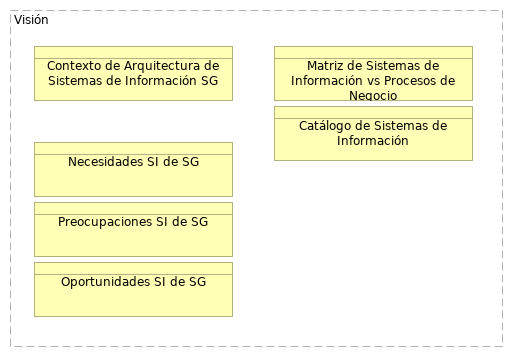
\includegraphics{images/03.EntregablesVision.png}
\caption{03. Entregables Vision. \emph{Fuente: Propuesta servicios de
ingeniería y evaluación de arquitectura Arquitectura de Aplicaciones
Secretaria de la Alcaldía de Bogotá
(2025)}}\label{fig:id-0993b3b264144f84abe5c7031666fede}
\end{figure}

\subsubsection{Visión}\label{sec:visiuxf3n}

\subsubsection{Contexto de Arquitectura de Sistemas de Información
SG}\label{sec:contexto-de-arquitectura-de-sistemas-de-informaciuxf3n-sg}

Desde el dominio de aplicaciones y sistemas de información de la
Secretaría General, llamada en adelante ``la arquitectura de sistemas de
Información de SG'', buscamos adelantar las especificaciones de las
arquitecturas objetivo de los sistemas de información de Secretaria de
la Alcaldía de Bogotá que soporten la arquitectura de negocio y datos,
en línea y dentro del alcance de la visión establecida en el primer
entregable de este ejercicio de arquitectura empresarial de SG (AESG).

En particular, la arquitectura de sistemas de información de SG se
plantea, dentro del alcance de la visión del ejercicio:

\begin{itemize}
\tightlist
\item
  Definir la arquitectura de las aplicaciones (SI) necesarias para
  soportar los procesos de negocio de SG.
\item
  Identificar las funciones de negocio que deben ser soportadas por las
  aplicaciones de SG.
\item
  Establecer la interacción y el flujo de información entre las
  diferentes aplicaciones de SG.
\item
  Considerar aspectos sistémicos como la escalabilidad, el rendimiento,
  la mantenibilidad y la seguridad de las aplicaciones de SG.
\item
  Listar los capacidades de negocio (servicios de aplicación)
  relacionadas con las arquitecturas de aplicaciones de SG.
\end{itemize}

De esta manera, la arquitectura de sistemas de SG contribuye a la
consecución de la visión de este ejercicio de arquitectura empresarial
SG (AESG); y en lo específico, contribuye a los fines de la arquitectura
de negocio y tecnológica de SG, a delinear oportunidades y soluciones, y
a soportar la planeación de la migración. Todo lo anterior dentro del
alcance consignado en este ejercicio.

\paragraph{Alcance}\label{sec:alcance}

El presente ejercicio de la arquitectura dominio de aplicaciones toma
como alcance horizontal las áreas o unidades siguientes de la SG
(\emph{fuente: sesiones de levantamiento, entrevistas, y cuestionarios
compartidos en el mes de julio del 2025, junto con la recopilación
estructurada de las fuentes de información y organigramas}):

Unidades de negocio del alcance del dominio:

\begin{itemize}
\tightlist
\item
  Secretaría Privada

  \begin{itemize}
  \tightlist
  \item
    Oficina Consejería Distrital de Comunicación. César Augusto Castro
    Rodríguez
  \item
    Oficina Consejería Distrital de Tecnologías de la Información y las
    Comunicaciones -TIC. Diana Celis Mora
  \end{itemize}
\item
  Despacho del Secretario General. Miguel Andrés Silva Moyano

  \begin{itemize}
  \tightlist
  \item
    Oficina de Tecnologías de la Información y las Comunicaciones.
    Arleth Patricia Saurith Contreras
  \item
    Subsecretaría Distrital de Fortalecimiento Institucional. Alejandra
    Rodas Gaiter

    \begin{itemize}
    \tightlist
    \item
      Dirección Distrital de Desarrollo Institucional. Sebastian Estrada
      Jaramillo

      \begin{itemize}
      \tightlist
      \item
        Subdirección Técnica de Desarrollo Institucional. Diego Canesco
        Arenas
      \end{itemize}
    \end{itemize}
  \item
    Subsecretaría de Servicio a la Ciudadanía . Adriana Vargas Tamayo

    \begin{itemize}
    \tightlist
    \item
      Dirección del Sistema Distrital de Servicio a la Ciudadanía.
      Enrique Cusba García
    \end{itemize}
  \item
    Subsecretaría Corporativa. Henry Villamarín Serrano
  \item
    Subsecreataría de Servicios Ciudadanos (\ldots)
  \item
    Subsecreataría de Inversión y FF (\ldots)
  \item
    Subsecreataría de Operaciones
  \item
    Subsecreataría de Relaciones Internacionales (\ldots)
  \end{itemize}
\end{itemize}

En cuanto al alcance vertical, las aplicaciones de software que están
consignadas en este ejercicio son las siguientes (\emph{fuente: sesiones
de levantamiento, entrevistas, y cuestionarios compartidos en el mes de
julio del 2025, junto con la recopilación estructurada de las fuentes de
información}):

\begin{itemize}
\tightlist
\item
  ADMON: Se relaciona con la gestión financiera, gestión de servicios
  administrativos y tecnológicos, y gestión de recursos físicos45.
\item
  Administrativo y Financiero: Soporta la gestión financiera, gestión de
  servicios administrativos y tecnológicos, y gestión de recursos
  físicos
\item
  Bogotá Te Escucha: Es fundamental para el proceso de Gobierno abierto
  y relacionamiento con la ciudadanía5. También se menciona como el
  Sistema Distrital para la Gestión de Peticiones Ciudadanas, a través
  del cual se evalúa la calidad de las respuestas emitidas a la
  ciudadanía
\item
  Bogotá Aprende TIC: Apoya los procesos de Gobierno abierto y
  relacionamiento con la ciudadanía, y Fortalecimiento de la Gestión
  Pública
\item
  DARUMA: Se utiliza en el proceso de Fortalecimiento de la Gestión
  Pública5. También es el aplicativo donde se encuentran definidas las
  fichas técnicas de productos y servicios de la Secretaría General8 y
  se gestionan los riesgos estratégicos
\item
  SIGA: Interviene en la gestión de contratación, gestión financiera,
  gestión de servicios administrativos y tecnológicos, y gestión de
  recursos físicos
\item
  SAT Web: Relacionado con la gestión de servicios administrativos y
  tecnológicos
\item
  GLOBO: Utilizado en el proceso de Fortalecimiento de la Gestión
  Pública
\item
  Datos para la Transparencia (SATI): Soporta el proceso de Gobierno
  abierto y relacionamiento con la ciudadanía
\item
  SUDIVC: Se aplica en los procesos de Gobierno abierto y
  relacionamiento con la ciudadanía, Paz, víctimas y reconciliación, y
  Fortalecimiento de la Gestión Pública
\item
  HUMANAPP: Apoya la gestión del talento humano
\item
  SIAB (El COFRE): Utilizado en los procesos de Gobierno abierto y
  relacionamiento con la ciudadanía, y Fortalecimiento de la Gestión
  Pública
\item
  KOHA: Relacionado con la Gestión del conocimiento
\item
  SIVIC: Interviene en los procesos de Paz, víctimas y reconciliación, y
  Fortalecimiento de la Gestión Pública
\item
  Data Warehouse AVANTI: Apoya la Gestión del conocimiento
\item
  Gestión Académica: Relacionado con la Gestión del conocimiento
\item
  EMLAZE: Utilizado en los procesos de Gobierno abierto y
  relacionamiento con la ciudadanía, y Fortalecimiento de la Gestión
  Pública
\item
  GLPI: Soporta la gestión de servicios administrativos y tecnológicos
\item
  GitLab: Se relaciona con la Gestión de alianzas e internacionalización
  de Bogotá
\end{itemize}

\subsubsection{Matriz de Sistemas de Información vs Procesos de
Negocio}\label{sec:matriz-de-sistemas-de-informaciuxf3n-vs-procesos-de-negocio}

Las matrices del dominio de aplicaciones de software y sistemas de
información (SI) de SG son herramientas para el relacionamiento con
otros dominios del ejercicio de arquitectura empresarial de SG. Con esto
conseguimos soportar la toma decisiones de lo que debe ser compartido de
los SI dentro de la Secretaría, y entre sus aplicaciones de software.
Las matrices de este ejercicio sirven además para comunicar el grado de
relacionamiento de los elementos.

En resumen,

\begin{itemize}
\tightlist
\item
  Las matrices son cruciales para especificar cómo debe relacionarse la
  información entre los sistemas y otros dominios
\item
  proporcionan información crítica para los proyectos que involucren a
  los sistemas de SG.
\item
  Contribuye a la determinación de brechas (gaps) en las necesidades de
  compartir información (o funciones de los sistemas) ente los elementos
  de la matriz.
\item
  La matriz ayuda a definir el nivel de detalle de lo que se comparte.
\item
  Se deben establecer medidas similares para la interoperabilidad de
  servicios/negocios y la infraestructura (tecnología física).
\item
  Sintetizan la información de las arquitecturas, y son simples para
  compartir documentos.
\end{itemize}

Las matrices de este dominio (procesos e interoperabilidad) actúan como
una hoja de ruta para la conectividad y el intercambio de información;
inician desde una perspectiva de negocio de alto nivel y van hasta una
especificación técnica detallada del la interacción con los sistemas.
Sirven como herramienta de comunicación para los demás dominios de la
arquitectura empresarial de SG, y contribuyen a que las interacciones
relevantes entre servicios, canales, y procesos estén definidas y sean
compatibles.

\subsubsection{Catálogo de Sistemas de
Información}\label{sec:catuxe1logo-de-sistemas-de-informaciuxf3n}

En el contexto de TOGAF, El Catálogo de sistemas de información es un
inventario detallado y documentado que actúa como ficha técnica de los
sistemas de información o aplicaciones de software de SG.

Es un producto entregable clave de la fase de Arquitectura de
Aplicaciones dentro de la Fase 3 de este ejercicio de arquitectura
empresarial (AE). Forma parte del Marco de Referencia del Contenido
Arquitectónico de TOGAF y del Marco de Arquitectura de Referencia del
MinTIC (MAE 3.0, Colombia).

La construcción del catálogo de aplicaciones implican a las sesiones de
levantamiento, entrevistas, y cuestionarios compartidos en el mes de
julio, junto con la recopilación estructurada de las fuentes de
información sobre cada sistema.

\paragraph{Contenido Mínimo del
Catálogo}\label{sec:contenido-muxednimo-del-catuxe1logo}

\begin{itemize}
\tightlist
\item
  ID de Aplicación. Código de identificación de la aplicación de
  software.
\item
  Nombre de la Aplicación. Nombre de identificación de la aplicación de
  software.
\item
  Descripción. Funcionamiento básico de la aplicación de software.
\item
  Estado: {[}En producción, en desmantelamiento, en implementación,
  Inactiva{]}
\item
  Categoría: {[}Sistema de apoyo al negocio (misional), herramienta de
  gestión, Ofimática, Seguridad{]}
\item
  Proceso(s) de Negocio Clave(s)
\item
  Capacidad: Capacidades de nivel 2 relacionadas con la aplicación de
  software.
\item
  Tipo de aplicación: Web, Móvil, Cliente Servidor
\item
  Método de despliegue: on-premises, cloud SAAS, cloud PAAS, cloud IAAS
\item
  Tecnología. Aspectos técnicos de la aplicación de software.
\item
  Versión actual de la tecnología
\item
  Responsable técnico en la entidad
\item
  Responsable funcional en la entidad
\item
  Fabricante
\item
  Proveedor de soporte externo
\item
  Fecha de vigencia de soporte externo
\item
  Nombre de servidor. Nombre de red del entorno o nodo contenedor de la
  aplicación de software.
\item
  Criticidad de negocio
\end{itemize}

El Catálogo de aplicaciones de SG procura beneficios estratégicos y
operativos:

\begin{itemize}
\tightlist
\item
  Unifica la documentación y la comunicación: Es un artefacto clave para
  documentar, comprender y comunicar el panorama actual y futuro de las
  aplicaciones.
\item
  Base para la toma de decisiones: Sirve como base para la toma de
  decisiones en la gestión y gobierno de las capacidades de los sistemas
  de SG, y del portafolio y ciclo de vida de las aplicaciones.
\item
  Facilita la actualización continua: Permite la actualización continua
  de las características y atributos relevantes de los sistemas de
  información.
\end{itemize}

\subsubsection{Necesidades SI de SG}\label{sec:necesidades-si-de-sg}

La construcción de lista de necesidades, preocupaciones y oportunidades
implican a las sesiones de levantamiento, entrevistas, y cuestionarios
compartidos en el mes de julio, junto con la recopilación estructurada
de las fuentes de información sobre cada sistema.

\paragraph{Necesidades de Transformación Digital y
Tecnológica}\label{sec:necesidades-de-transformaciuxf3n-digital-y-tecnoluxf3gica}

La transformación digital (objetivo estratégico de SG) es un motor
fundamental para alinear las estrategias, procesos y tecnologías de la
Secretaría General. Esta transformación busca:

\begin{itemize}
\item
  Impulsar la transformación digital para alinear estrategias, procesos
  y tecnologías, que resulte en el aumento de eficiencia de la gestión
  pública.
\item
  Cerrar las brechas en la Política de Gobierno Digital, de la cual la
  Arquitectura Empresarial es un habilitador clave.
\item
  Modernizar la infraestructura tecnológica que resulte del análisis de
  obsolescencia para asegurar su continuidad y disponibilidad.
\item
  Integrar plataformas y ecosistemas digitales y superar la falta de
  interoperabilidad.
\item
  Aumentar la automatización de los trámites digitales.
\item
  Estandarizar la gestión y gobernanza de datos públicos.
\item
  Mejorar el soporte que los SI dan a la toma de decisiones basada en
  evidencia.
\item
  Generar análisis predictivos y prospectivos de resultados de gestión,
  que son insumos para la toma de decisiones.
\item
  Contar con disponibilidad de personal adecuado para actualizar
  plataformas tecnológicas y gestionar las cargas de trabajo.
\item
  Aprovechar nuevas tecnologías como la Inteligencia Artificial, la
  minería de datos, el procesamiento del lenguaje, para mejorar los
  procesos y la relación con la ciudadanía.
\item
  Abordar los altos costos de la tecnología que limitan la
  implementación de sistemas avanzados. (??)
\item
  Fortalecer la ciberseguridad y seguridad de la información para
  proteger la integridad, disponibilidad y confidencialidad de los datos
  y prevenir ataques.
\end{itemize}

\paragraph{Necesidades Específicas del Dominio de Aplicaciones de
software}\label{sec:necesidades-especuxedficas-del-dominio-de-aplicaciones-de-software}

Esta tipo de necesidades refiere al comportamiento de las aplicaciones
que apoyan la misionalidad, a su estructura, y su relación con los
objetos de datos que utilizan.

Para los Componentes de Aplicación (Application Component) y Servicios
de Aplicación (Application Service) de SG:

\begin{itemize}
\tightlist
\item
  Adquirir software especializado en análisis de datos: implica la
  necesidad de incorporar de nuevos componentes de aplicación
  (Application Component).
\item
  Integrar plataformas y ecosistemas digitales :requiere reforzar la
  relación entre componentes de aplicación y la exposición de servicios
  de aplicación (Application Service), y clicar los lineamientos del
  Marco de Referencia de AE, versión 3.0 al momento, del MinTIC.
\item
  Mejorar la capacidad de las herramientas tecnológicas para el soporte
  a la toma de decisiones y la gestión: requiere la mejora de las
  Funcionalidad (Application Function) y Componentes de Aplicación
  actuales asociadas a esta capacidad.
\end{itemize}

\subsubsection{Preocupaciones SI de
SG}\label{sec:preocupaciones-si-de-sg}

Con base en el estudio de las sesiones de levantamiento, entrevistas, y
cuestionarios compartidos en el mes de julio, junto con la recopilación
estructurada de las fuentes de información sobre cada sistema,
identificamos las siguientes preocupaciones (y debilidades) de SG
relacionadas con el dominio de sistemas de información, dentro del
alcance de este ejercicio.

Las preocupaciones tecnológicas respecto de los sistemas de información
de SG mencionadas en estas fuentes señalan:

\begin{itemize}
\tightlist
\item
  Deficiente apropiación del conocimiento en procesos de tecnologías de
  la información, lo que genera demora en la solución de los servicios
  de tecnologías de la información.
\item
  Equipos tecnológicos en proceso de mitigar la obsolescencia, que
  generan dificultad en la ejecución de las actividades que desarrolla
  la entidad.
\item
  Fallas recurrentes en el funcionamiento de los sistemas de información
  y plataformas tecnológicas de la entidad, que afectan la continuidad
  del servicio y generan retrasos y reprocesos en la ejecución de las
  actividades.
\item
  Insuficiencia en la capacidad de las herramientas tecnológicas de la
  entidad que pueden obstaculizar el avance de los iniciativas en marcha
  de la SG.
\item
  Debilidad en la capacidad de extraer información dinámica que sirva
  como insumo para la toma de decisiones basado en evidencia.
\item
  Se realizan análisis de datos descriptivos aislados, pero no
  predictivos y prospectivos de los resultados de la gestión de la
  entidad, lo que dificulta la toma de decisiones basada en evidencia.
\item
  Falta de personal para actualizar las plataformas tecnológicas, lo que
  genera retrasos en la operación de la entidad.
\item
  Deficiente conectividad y falta de interoperabilidad de las
  plataformas tecnológicas.
\item
  Cambios en las plataformas tecnológicas que no interactúan con las
  anteriores, lo cual expone a la SG a posibles pérdidas de información
  y reprocesos.
\item
  Apostar más en la mejora continua de la inestabilidad de la
  conectividad, indisponibilidad de servidores de información y
  vulnerabilidad en la seguridad informática; lo contrario puede
  comprometer la operatividad, la integridad de los datos críticos de la
  entidad y el cumplimiento de las metas.
\item
  Potencial y rápida obsolescencia tecnológica que implica la necesidad
  de renovación de los equipos y dificulta la prestación de los
  servicios de la entidad.
\item
  Los altos costos de la tecnología pueden limitar la capacidad de la
  entidad para implementar y mantener sistemas avanzados y eficientes.
\end{itemize}

\subsubsection{Oportunidades SI de SG}\label{sec:oportunidades-si-de-sg}

La construcción de lista de oportunidades mencionadas implica el estudio
de las sesiones de levantamiento, entrevistas, y cuestionarios
compartidos en el mes de julio, junto con la recopilación estructurada
de las fuentes de información al respecto de cada sistema de SG.

Las oportunidades tecnológicas y de mejora de sistemas de información
mencionadas indicadas en estas fuentes se centran en:

\begin{itemize}
\item
  Modernización de la infraestructura y sistemas tecnológicos

  \begin{itemize}
  \tightlist
  \item
    Las nuevas tecnologías, especialmente la Inteligencia Artificial
    (IA), ofrecen la oportunidad de mejorar los procesos y herramientas
    de relacionamiento con la ciudadanía. La Secretaría General ya ha
    empezado a incorporar tecnologías como IA, Big Data, pero debe
    seguir ampliando ese despliegue, así como incorporar otras, como el
    Internet de las Cosas (IoT), o la minería de datos en la
    planificación urbana y la prestación de servicios.
  \item
    Una oportunidad es la adquisición y puesta en producción de software
    especializado en análisis de datos para la toma de decisiones que ya
    poseen otras entidades.
  \end{itemize}
\item
  Integración y automatización de procesos

  \begin{itemize}
  \tightlist
  \item
    Se identifican oportunidades para contar con herramientas que
    evalúen el soporte tecnológico personalizado, flexible y
    configurable para las operaciones de los procesos jurídicos.
  \item
    Se buscan mejores controles e integración de sistemas distritales
    con los canales de la Secretaría General.
  \item
    También se necesitan mejores controles e integración de los sistemas
    de gestión como los sistemas GLOBO (de gestión internacional), el
    sistema de proyectos GLPI.
  \end{itemize}
\item
  Mejora de la comunicación pública a través de medios digitales

  \begin{itemize}
  \tightlist
  \item
    Se busca la consolidación de herramientas, canales e información
    para fortalecer la oferta y celeridad de servicios y la
    participación ciudadana. Esto incluye el seguimiento a canales de
    atención virtual como SuperCADE Virtual, chat, chat-Bot y (video)
    llamadas de la línea 195.
  \item
    Se busca optimizar los procesos de recolección, análisis y
    divulgación de la información mediante la implementación de sistemas
    de información que incluyan la automatización de la recolección de
    datos y el uso de herramientas analíticas.
  \item
    Es destacado que el Distrito unifica en el portal Bogotá su oferta
    de trámites y servicios, como el realizar pagos en línea (no
    tributarios) y agendamiento de citas en la RedCADE desde casa;
    esfuerzo que debe continuar y extenderse a los más de 1.400 trámites
    y servicios. Esto representa una mejora significativa en la
    accesibilidad y eficiencia de los servicios digitales para la
    ciudadanía.
  \end{itemize}
\item
  capacitación en nuevas tecnologías y
\item
  Implementación de la Arquitectura Empresarial como estrategia para
  impulsar la transformación digital y la eficiencia en la gestión
  pública de la SG

  \begin{itemize}
  \tightlist
  \item
    Se espera que la Arquitectura Empresarial fortalezca la
    transparencia, y aumente la eficiencia de la gestión pública y la
    rendición de cuentas al estandarizar procesos y sistemas de
    información. La AE busca realmente impactar el objetivo de aumentar
    la confianza de la ciudadanía en la Gestión Pública.
  \item
    Es requerido que este ejercicio beneficie a la SG con la entrega de
    activos como hojas de ruta, catálogos y caracterización de los
    sistemas de información, matrices de interacción, entre otros.
  \end{itemize}
\end{itemize}

\newpage

\section{Documentación del Dominio de
Aplicaciones}\label{sec:documentaciuxf3n-del-dominio-de-aplicaciones}

\subsection{SI del Análisis de
Entorno}\label{sec:si-del-anuxe1lisis-de-entorno}

\begin{quote}
Desafíos operativos que justifican la existencia y la necesidad de
optimización e integración de todos los sistemas de información del
Anexo Técnico SG.
\end{quote}

El ``Anexo Técnico ADENDA.pdf'' detalla la consultoría para implementar
la Arquitectura Empresarial, que busca fortalecer la alineación de
estrategias, procesos y tecnologías, así como impulsar la transformación
digital y una gestión pública más eficiente. Esta iniciativa se enmarca
en la necesidad de mejorar la satisfacción de los grupos de interés
internos y externos.

El ``Resumen Ejecutivo FASE I.pdf'' contextualiza estos esfuerzos al
analizar el entorno de la gestión pública distrital, identificando
brechas, tendencias y oportunidades a través de factores
político-institucionales, económicos, sociales, tecnológicos, ecológicos
y legales.

Las relaciones entre los sistemas de información mencionados en el Anexo
Técnico y el contexto del Análisis de Entorno (Resumen Ejecutivo FASE
I.pdf) son las siguientes:

\begin{itemize}
\tightlist
\item
  Sistemas de gestión administrativa y financiera (ADMON, Administrativo
  y Financiero, SIGA, SAT Web, GLPI):

  \begin{itemize}
  \tightlist
  \item
    Estos sistemas son cruciales para la ``Gestión financiera'',
    ``Gestión de servicios administrativos y tecnológicos'' y ``Gestión
    de recursos físicos''.
  \item
    Relación con objetivos: El ``Resumen Ejecutivo FASE I.pdf'' aborda
    la necesidad de una gestión pública más eficiente y transparente, la
    optimización de recursos y la rendición de cuentas. Estos sistemas
    son habilitadores directos de dichas metas.
  \item
    Relación con problemas: El documento también señala desafíos en el
    ``Entorno Económico'' como el déficit fiscal y la necesidad de
    eficiencia en la inversión pública. Los sistemas administrativos y
    financieros son fundamentales para una planificación financiera
    adecuada y una gestión fiscal sostenible.
  \item
    Relación con oportunidades: La recomendación de ``simplificación
    administrativa y coordinación intersectorial'' implica la mejora de
    estos sistemas para reducir duplicidades y estandarizar prácticas,
    lo que contribuye a una ``arquitectura institucional más coherente y
    eficiente''.
  \end{itemize}
\item
  Sistemas de interacción ciudadana y transparencia (Bogotá Te Escucha,
  Datos para la Transparencia (SATI), EMLAZE):

  \begin{itemize}
  \tightlist
  \item
    Estos sistemas soportan directamente el proceso de ``Gobierno
    abierto y relacionamiento con la ciudadanía''.
  \item
    Objetivos: El ``Resumen Ejecutivo FASE I.pdf'' destaca el objetivo
    estratégico ``Bogotá confía en su gobierno'', que busca ofrecer
    ``servicios amables, ágiles y oportunos''. Bogotá Te Escucha es el
    sistema distrital clave para la gestión de peticiones ciudadanas y
    la evaluación de la calidad de las respuestas.
  \item
    Problemas: Se reconoce que, si bien hay avances en la atención
    institucional, persisten desafíos en la ``eficiencia operativa,
    tiempos de respuesta y digitalización de servicios''. Estos sistemas
    son vitales para abordar estas brechas mediante la digitalización de
    servicios públicos y la automatización de trámites.
  \item
    Oportunidad: ``Datos para la Transparencia (SATI)'' es clave para la
    política de ``Transparencia, acceso a la información pública y lucha
    contra la corrupción''. La estandarización de procesos y sistemas de
    información a través de estos sistemas fortalece la confianza
    ciudadana.
  \end{itemize}
\item
  Sistemas de fortalecimiento de capacidades y conocimiento (Bogotá
  Aprende TIC, DARUMA, GLOBO, SUDIVC, HUMANAPP, SIAB (El COFRE), KOHA,
  SIVIC, Data Warehouse AVANTI, Gestión Académica):
\end{itemize}

\paragraph{Relación con Objetivos}\label{sec:relaciuxf3n-con-objetivos}

\begin{verbatim}
- Bogotá Aprende TIC y Gestión Académica abordan la necesidad de "alfabetización digital" y la escasez de talento humano especializado en tecnologías emergentes, como se menciona en el "Entorno Tecnológico".
- DARUMA es el aplicativo donde se gestionan las fichas técnicas de productos y servicios y los riesgos estratégicos. Esto se alinea con la necesidad de una "Gestión del riesgo" efectiva y el "Fortalecimiento de la Gestión Pública" para la toma de decisiones basada en evidencia.
- HUMANAPP es fundamental para la "Gestión del talento humano". El "Resumen Ejecutivo FASE I.pdf" subraya la importancia de la "profesionalización del servicio público" y el "fortalecimiento de capacidades" de los servidores públicos.
- SIAB (El COFRE), KOHA, Data Warehouse AVANTI son cruciales para la "Gestión del conocimiento" y la "Gestión documental y soporte archivístico". El documento enfatiza el "fortalecimiento de las capacidades de generación, análisis y uso estratégico de información" y la necesidad de "sistemas integrados de datos" para la toma de decisiones basada en evidencia. Data Warehouse AVANTI, en particular, facilita el análisis descriptivo, predictivo y prospectivo de los resultados de la gestión.
- SUDIVC y SIVIC apoyan los procesos de "Paz, víctimas y reconciliación" y "Fortalecimiento de la Gestión Pública", abordando las "profundas desigualdades que afectan de manera desproporcionada a poblaciones vulnerables" y contribuyendo a que Bogotá sea un "territorio de paz y reconciliación".
\end{verbatim}

\begin{itemize}
\tightlist
\item
  Sistemas de desarrollo y colaboración (GitLab):
\end{itemize}

\paragraph{Relación con
Oportunidades}\label{sec:relaciuxf3n-con-oportunidades}

\begin{verbatim}
- GitLab, siendo una plataforma de desarrollo y colaboración, está vinculada con la "Gestión de alianzas e internacionalización de Bogotá".
- El "Resumen Ejecutivo FASE I.pdf" menciona la consolidación de Bogotá como una ciudad con "vocación internacional, atrayendo a profesionales, diplomáticos, académicos y organizaciones" y la necesidad de "fortalecer la arquitectura Internacional del Distrito". GitLab puede ser una herramienta para facilitar la colaboración en proyectos y la gestión de información en el marco de estas alianzas.
- También se alinea con la necesidad de "integración entre plataformas digitales institucionales" y la adopción de nuevas tecnologías para la "transformación digital".
\end{verbatim}

En síntesis, el ``Resumen Ejecutivo FASE I.pdf'' proporciona el marco
estratégico y los desafíos operativos que justifican la existencia y la
necesidad de optimización e integración de todos los sistemas de
información mencionados en el ``Anexo Técnico ADENDA.pdf''. El ejercicio
de Arquitectura Empresarial busca cerrar las brechas identificadas y
avanzar hacia una gestión pública más eficiente, transparente, digital y
centrada en el ciudadano, aprovechando al máximo sus sistemas y
tecnologías.

\begin{figure}
\centering
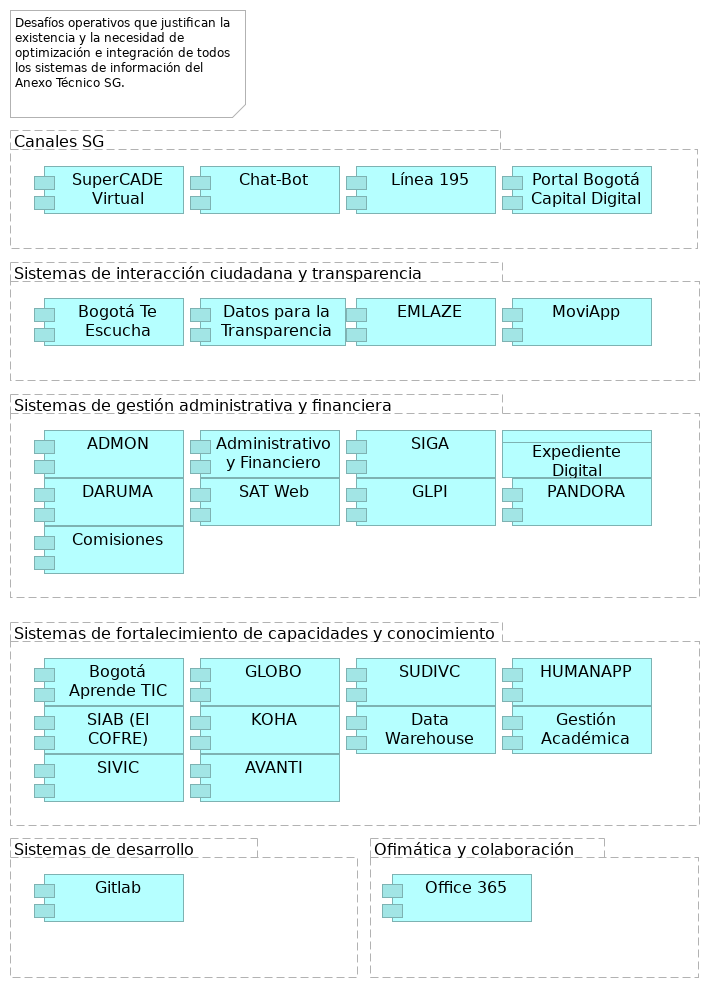
\includegraphics{images/06.2n2.SIdelAnalisisdeEntorno.png}
\caption{06.2n2. SI del Analisis de Entorno. \emph{Fuente: Propuesta
servicios de ingeniería y evaluación de arquitectura Arquitectura de
Aplicaciones Secretaria de la Alcaldía de Bogotá
(2025)}}\label{fig:id-097745511d984e7eaf02b5ad5a93e7a8}
\end{figure}

\subsubsection{Canales SG}\label{sec:canales-sg}

\subsubsection{Portal Bogotá Capital
Digital}\label{sec:portal-bogotuxe1-capital-digital}

Portal Integrador de trámites y servicios ofrecidos a la ciudadanía.
\#\#\# Sistemas de interacción ciudadana y transparencia

\subsubsection{MoviApp}\label{sec:moviapp}

Sesión levantamiento no. 2. \#\#\# Sistemas de gestión administrativa y
financiera

\subsubsection{Expediente Digital}\label{sec:expediente-digital}

Objeto de datos en la capa de aplicación que representa un expediente
electrónico. \#\#\# PANDORA Implementación de temas precontractual y
planeación. \#\#\# Comisiones Sesión levantamiento no. 1.

\subsubsection{Sistemas de fortalecimiento de capacidades y
conocimiento}\label{sec:sistemas-de-fortalecimiento-de-capacidades-y-conocimiento}

\subsubsection{SIAB (El COFRE)}\label{sec:siab-el-cofre}

Sistema de Información del Archivo de Bogotá SIAB. Permite automatizar
los procesos archivísticos y técnicos que realiza el Archivo, tales como
llevar un registro de los Ingresos Documentales (antes área de acopio),
para la descripción y catalogación de la documentación, propios del
proceso de Gestión de la Función Archivística y del Patrimonio
Documental, para su custodia y conservación permanente. \#\#\# AVANTI
Apoya la Gestión del conocimiento.

\subsubsection{Sistemas de desarrollo}\label{sec:sistemas-de-desarrollo}

\subsubsection{Ofimática y
colaboración}\label{sec:ofimuxe1tica-y-colaboraciuxf3n}

\subsection{Objetivos Estratégicos
SG-OTIC}\label{sec:objetivos-estratuxe9gicos-sg-otic}

\begin{quote}
\end{quote}

Alineación entre los objetivos estratégicos de la Secretaría General de
la Alcaldía Mayor de Bogotá D.C. (SG) y los objetivos de la Oficina de
Tecnologías de la Información y las Comunicaciones (OTIC). \emph{Muestra
cómo los esfuerzos de TI (objetivos accionables, personas y procesos e
iniciativas) habilitan las metas institucionales de alto nivel}.

\begin{figure}
\centering
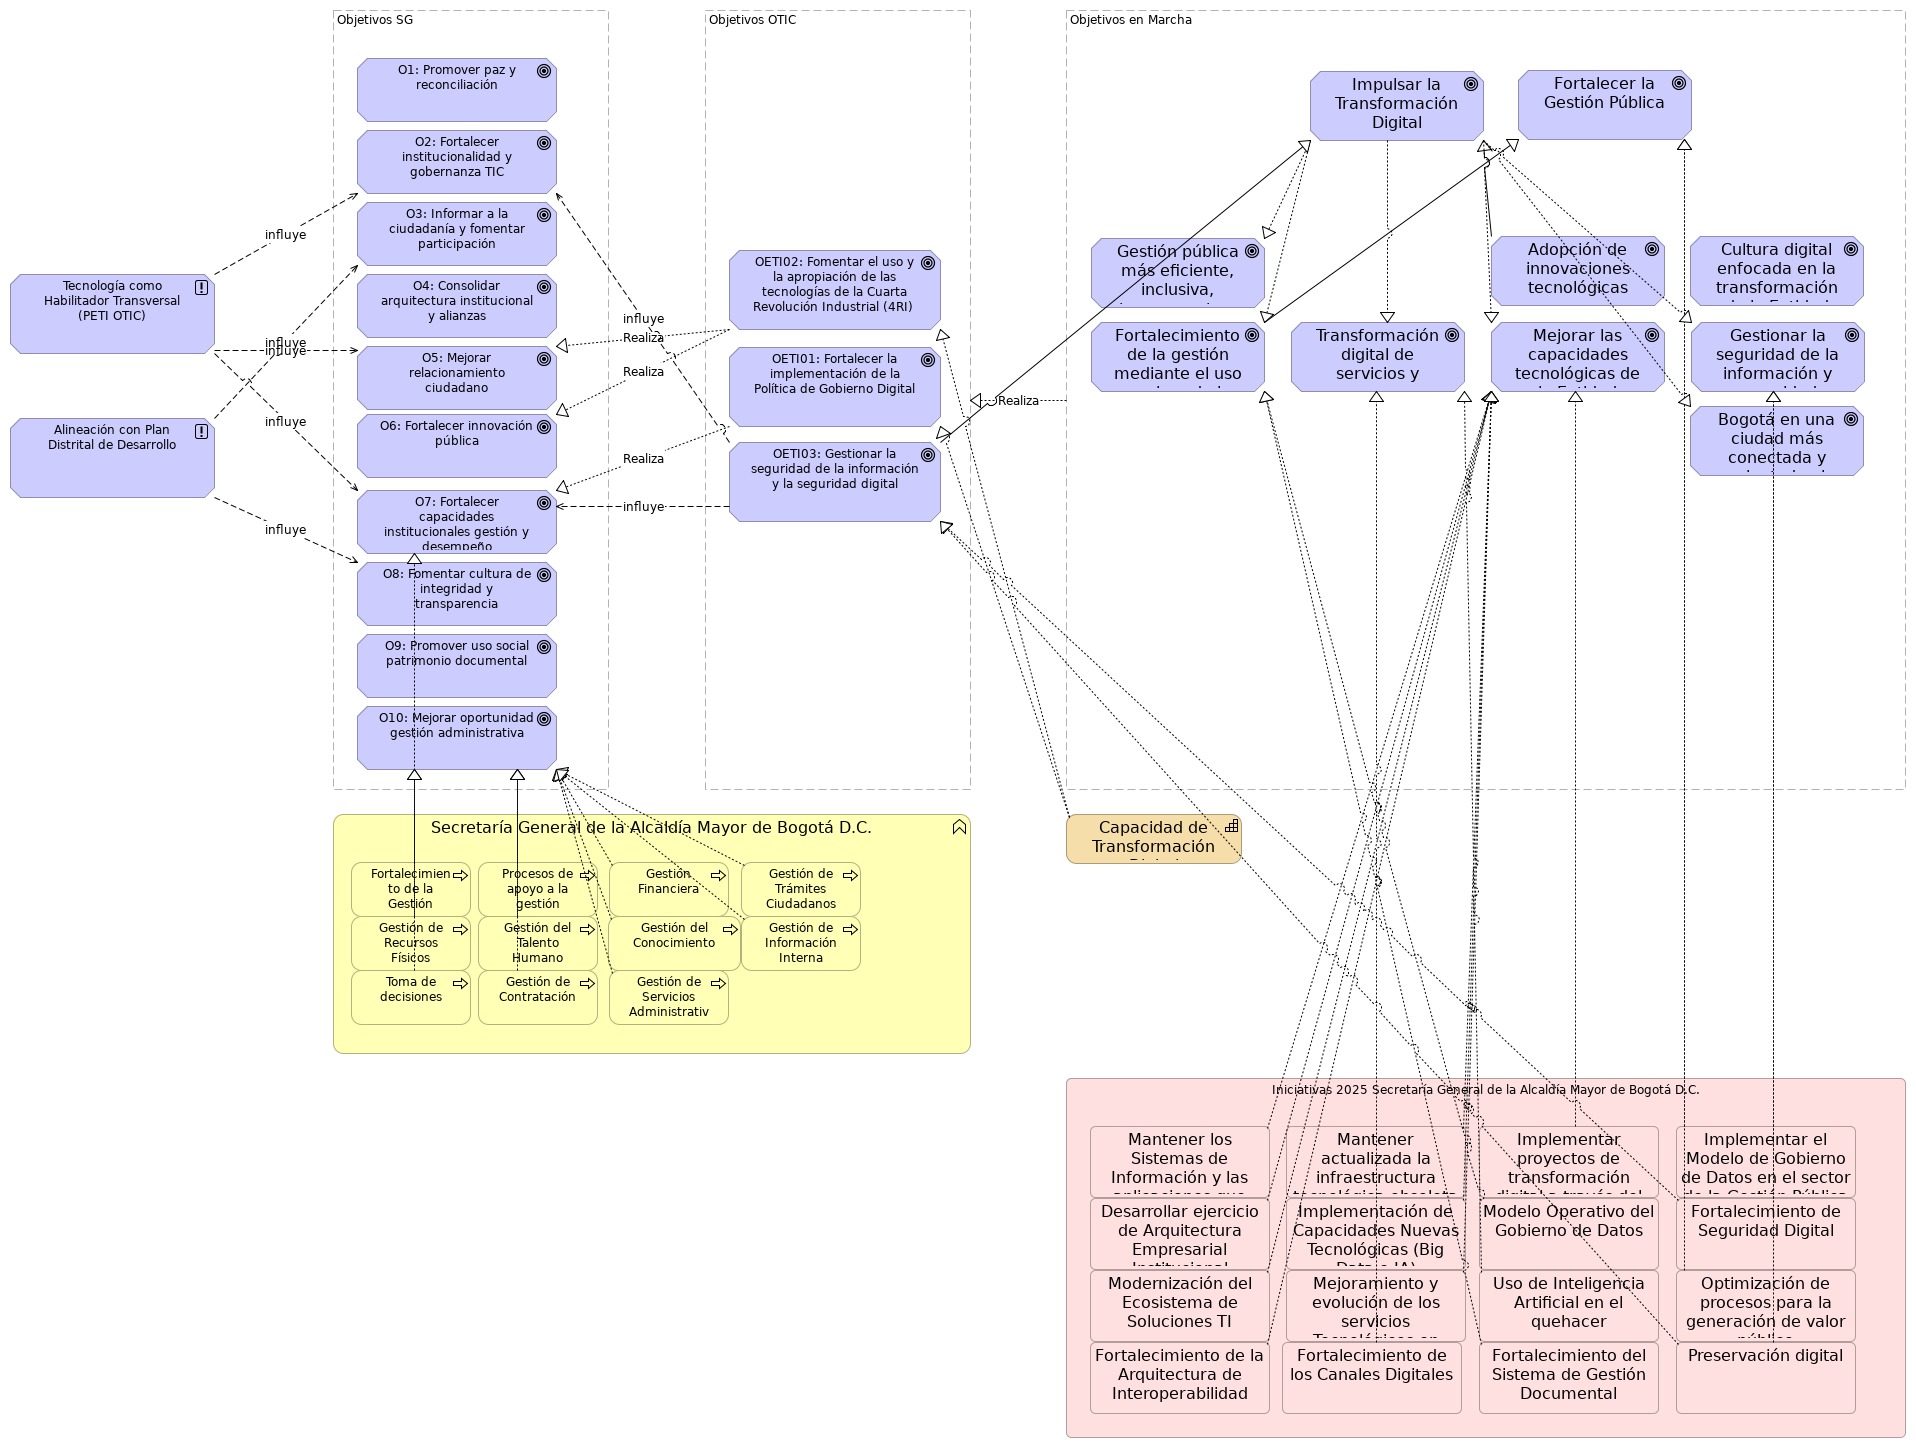
\includegraphics{images/06.BMM.ObjetivosEstrategicosSG-OTIC.png}
\caption{06.BMM. Objetivos Estrategicos SG-OTIC. \emph{Fuente: Propuesta
servicios de ingeniería y evaluación de arquitectura Arquitectura de
Aplicaciones Secretaria de la Alcaldía de Bogotá
(2025)}}\label{fig:id-257a9a842fe0459c88cf09c4ebd37805}
\end{figure}

\subsubsection{Objetivos SG}\label{sec:objetivos-sg}

\subsubsection{O1: Promover paz y
reconciliación}\label{sec:o1-promover-paz-y-reconciliaciuxf3n}

Promover la paz y la reconciliación en Bogotá a través de la integración
local de las poblaciones afectadas por el conflicto armado, buscando la
superación de sus condiciones de vulnerabilidad y la reconstrucción del
tejido social en la ciudad. \#\#\# O2: Fortalecer institucionalidad y
gobernanza TIC Fortalecer la institucionalidad y gobernanza para
impulsar y coordinar el uso de las Tecnologías de la Información y las
Comunicaciones (TIC), con el fin de establecer un marco normativo,
habilitar la infraestructura, promover el talento digital y crear
procesos eficientes para la prestación de servicios ciudadanos y la
transformación de la administración pública. \#\#\# O3: Informar a la
ciudadanía y fomentar participación Informar a la ciudadanía mediante
campañas y estrategias de comunicación sobre temas de ciudad, para
fomentar la participación ciudadana y la transparencia de la gestión
pública. \#\#\# O4: Consolidar arquitectura institucional y alianzas
Desarrollar y consolidar la arquitectura institucional, los instrumentos
de política pública y las alianzas estratégicas necesarias para
posicionar a Bogotá como una ciudad globalmente accesible y abierta al
mundo. \#\#\# O5: Mejorar relacionamiento ciudadano Mejorar el
relacionamiento de la ciudadanía con el gobierno distrital a través del
fortalecimiento de la oferta institucional, la modernización de los
canales de atención y la cualificación del talento humano, contribuyendo
al aumento de la confianza y satisfacción ciudadana. \#\#\# O6:
Fortalecer innovación pública Fortalecer los procesos de innovación
pública en las entidades distritales, facilitando habilitadores,
desarrollando capacidades en intraemprendimiento, promoviendo el trabajo
colaborativo y la articulación entre actores públicos y privados. \#\#\#
O7: Fortalecer capacidades institucionales gestión y desempeño
Fortalecer las capacidades institucionales para la implementación de las
políticas de gestión y desempeño, con el objetivo de generar valor
público, contribuir a la solución de los retos de la ciudad y promover
la participación ciudadana. \#\#\# O8: Fomentar cultura de integridad y
transparencia Fomentar una cultura de integridad, transparencia y ética
pública en la Administración Distrital. \#\#\# O9: Promover uso social
patrimonio documental Promover la apropiación y uso social del
patrimonio documental del Distrito Capital, mediante su protección,
conservación, adecuada gestión y fácil acceso por parte de la
ciudadanía. \#\#\# O10: Mejorar oportunidad gestión administrativa
Mejorar la oportunidad en la gestión administrativa, garantizando la
adquisición de bienes y servicios que satisfagan las necesidades de la
entidad y la ciudadanía, en el marco de la optimización de los recursos
asignados. \#\#\# Objetivos OTIC

\subsubsection{OETI02: Fomentar el uso y la apropiación de las
tecnologías de la Cuarta Revolución Industrial
(4RI)}\label{sec:oeti02-fomentar-el-uso-y-la-apropiaciuxf3n-de-las-tecnologuxedas-de-la-cuarta-revoluciuxf3n-industrial-4ri}

Fomentar el uso y la apropiación de las tecnologías de la Cuarta
Revolución Industrial (4RI) para impulsar la transformación digital en
la Secretaría General, integrando tecnologías emergentes que optimicen
los procesos, promuevan la innovación y mejoren la eficiencia en la
gestión pública. \#\#\# OETI01: Fortalecer la implementación de la
Política de Gobierno Digital Fortalecer la implementación de la Política
de Gobierno Digital para promover la transformación digital en la
Secretaría General, y optimizar las capacidades tecnológicas, con el fin
de garantizar una gestión pública eficiente, transparente y accesible
para la ciudadanía. \#\#\# OETI03: Gestionar la seguridad de la
información y la seguridad digital Gestionar la seguridad de la
información y la seguridad digital mediante la adopción de políticas,
controles y campañas de concienciación que fomenten una cultura digital
segura, así como la implementación de estrategias para asegurar la
continuidad de los servicios de TIC. \#\#\# Objetivos en Marcha

\subsubsection{Fortalecer la Gestión
Pública}\label{sec:fortalecer-la-gestiuxf3n-puxfablica}

Objetivo de TI de alto nivel optimizar (mejorar la eficiencia y
eficacia) los procesos y servicios de la administración pública.

\subsubsection{Impulsar la Transformación
Digital}\label{sec:impulsar-la-transformaciuxf3n-digital}

Meta principal del PETI, buscando modernizar la entidad a través de
tecnologías digitales. Contiene a la Política de Gobierno Digital.
\#\#\# Adopción de innovaciones tecnológicas para apoyar áreas
misionales clave Objetivo de integrar nuevas tecnologías para mejorar
funciones principales. \#\#\# Cultura digital enfocada en la
transformación de la Entidad Meta de fomentar una mentalidad y
habilidades digitales dentro de la organización. \#\#\# Gestión pública
más eficiente, inclusiva, transparente y confiable Resultado deseado de
una administración pública mejorada para los ciudadanos. \#\#\#
Fortalecimiento de la gestión mediante el uso y mejora de las
tecnologías Objetivo de mejorar la gestión pública mediante la
aplicación de TI. \#\#\# Transformación digital de servicios y procesos
administrativos Meta de digitalizar y optimizar los servicios y procesos
internos y externos. \#\#\# Mejorar las capacidades tecnológicas de la
Entidad (objetivo estratégico de TI) Meta de TI para modernizar y
potenciar la infraestructura y habilidades tecnológicas. \#\#\#
Gestionar la seguridad de la información y seguridad digital (objetivo
estratégico de TI) Objetivo de TI para proteger los activos de
información y garantizar la ciberseguridad. \#\#\# Bogotá en una ciudad
más conectada y orientada al bienestar de la ciudadanía Visión a largo
plazo para la ciudad impulsada por la digitalización. \#\#\# Tecnología
como Habilitador Transversal (PETI OTIC) El PETI de la OTIC busca que la
tecnología sea un habilitador transversal para una gestión pública más
eficiente, inclusiva, transparente y confiable, optimizando los trámites
y servicios ofrecidos a la ciudadanía. Para ello, la integración de las
tecnologías debe estar alineada con el direccionamiento estratégico y la
planeación institucional de la Entidad. \#\#\# Alineación con Plan
Distrital de Desarrollo El PETI está alineado con las políticas y
lineamientos del Plan Distrital de Desarrollo ``Bogotá camina segura
2024-2027'', especialmente con su Objetivo 5: ``Bogotá confía en su
gobierno'', que busca promover la confianza en la administración
distrital. \#\#\# Secretaría General de la Alcaldía Mayor de Bogotá D.C.
Entidad principal de la administración distrital. \#\#\# Procesos de
apoyo a la gestión Procesos internos que facilitan la operación de la
entidad. \#\#\# Gestión de Trámites Ciudadanos Proceso de atención y
resolución de solicitudes y gestiones de los ciudadanos. \#\#\# Gestión
de Información Interna Proceso de recolección, procesamiento y
distribución de información dentro de la entidad. \#\#\# Toma de
decisiones Proceso fundamental para la dirección estratégica y operativa
de la entidad. \#\#\# Capacidad de Transformación Digital Habilidad de
la entidad para adaptarse y evolucionar digitalmente. \#\#\# Mantener
los Sistemas de Información y las aplicaciones que apalanquen los
procesos misionales y de apoyo a la gestión Actividad continua para
asegurar la operatividad y soporte de los sistemas de información clave.
\#\#\# Mantener actualizada la infraestructura tecnológica obsoleta
Proyecto recurrente para asegurar la modernización y sostenibilidad de
la infraestructura de TI. \#\#\# Implementar proyectos de transformación
digital a través del uso de Tecnologías de Cuarta Revolución Industrial
(4RI) Ejecución de iniciativas que adoptan tecnologías avanzadas para la
transformación digital. \#\#\# Implementar el Modelo de Gobierno de
Datos en el sector de la Gestión Pública Proyecto para poner en práctica
el marco de gobernanza de datos en el ámbito público. \#\#\# Desarrollar
ejercicio de Arquitectura Empresarial Institucional Proyecto para
establecer y madurar la práctica de Arquitectura Empresarial en la
entidad. \#\#\# Implementación de Capacidades Nuevas Tecnológicas (Big
Data e IA) Iniciativa para incorporar tecnologías emergentes de la
Cuarta Revolución Industrial para optimizar procesos, impulsar la
innovación y garantizar la transformación digital. \#\#\# Modelo
Operativo del Gobierno de Datos Proyecto para definir e implementar un
marco de gobernanza de datos. \#\#\# Fortalecimiento de Seguridad
Digital Iniciativa para proteger la infraestructura y los datos de
amenazas digitales. \#\#\# Modernización del Ecosistema de Soluciones TI
Proyecto para actualizar y optimizar el conjunto de soluciones
tecnológicas. \#\#\# Mejoramiento y evolución de los servicios
Tecnológicos en Nube Iniciativa para optimizar y expandir el uso de
servicios cloud. \#\#\# Uso de Inteligencia Artificial en el quehacer
Proyecto para integrar la IA en las operaciones diarias de la entidad.
\#\#\# Optimización de procesos para la generación de valor público
Proyecto para revisar y mejorar los procesos internos con foco en el
valor para el ciudadano. \#\#\# Fortalecimiento de la Arquitectura de
Interoperabilidad Iniciativa para mejorar la comunicación e integración
entre sistemas y entidades. \#\#\# Fortalecimiento de los Canales
Digitales Iniciativa para mejorar la calidad y alcance de los canales de
atención digitales. \#\#\# Fortalecimiento del Sistema de Gestión
Documental Iniciativa para el desarrollo e implementación de
herramientas y procesos avanzados para optimizar la clasificación,
almacenamiento, acceso y control de la documentación institucional.
\#\#\# Preservación digital Proyecto para asegurar la conservación y
accesibilidad a largo plazo de los activos digitales.

\subsection{Objetivos e Iniciativas. PETI
SG}\label{sec:objetivos-e-iniciativas.-peti-sg}

\begin{quote}
\end{quote}

Diagrama que muestra la alineación estratégica, los actores de negocio y
los principales componentes de aplicación relacionados con la
Transformación Digital de la Alcaldía Mayor de Bogotá D.C. Se enfoca en
la trazabilidad desde las metas estratégicas hasta los proyectos y los
sistemas de información.

\begin{figure}
\centering
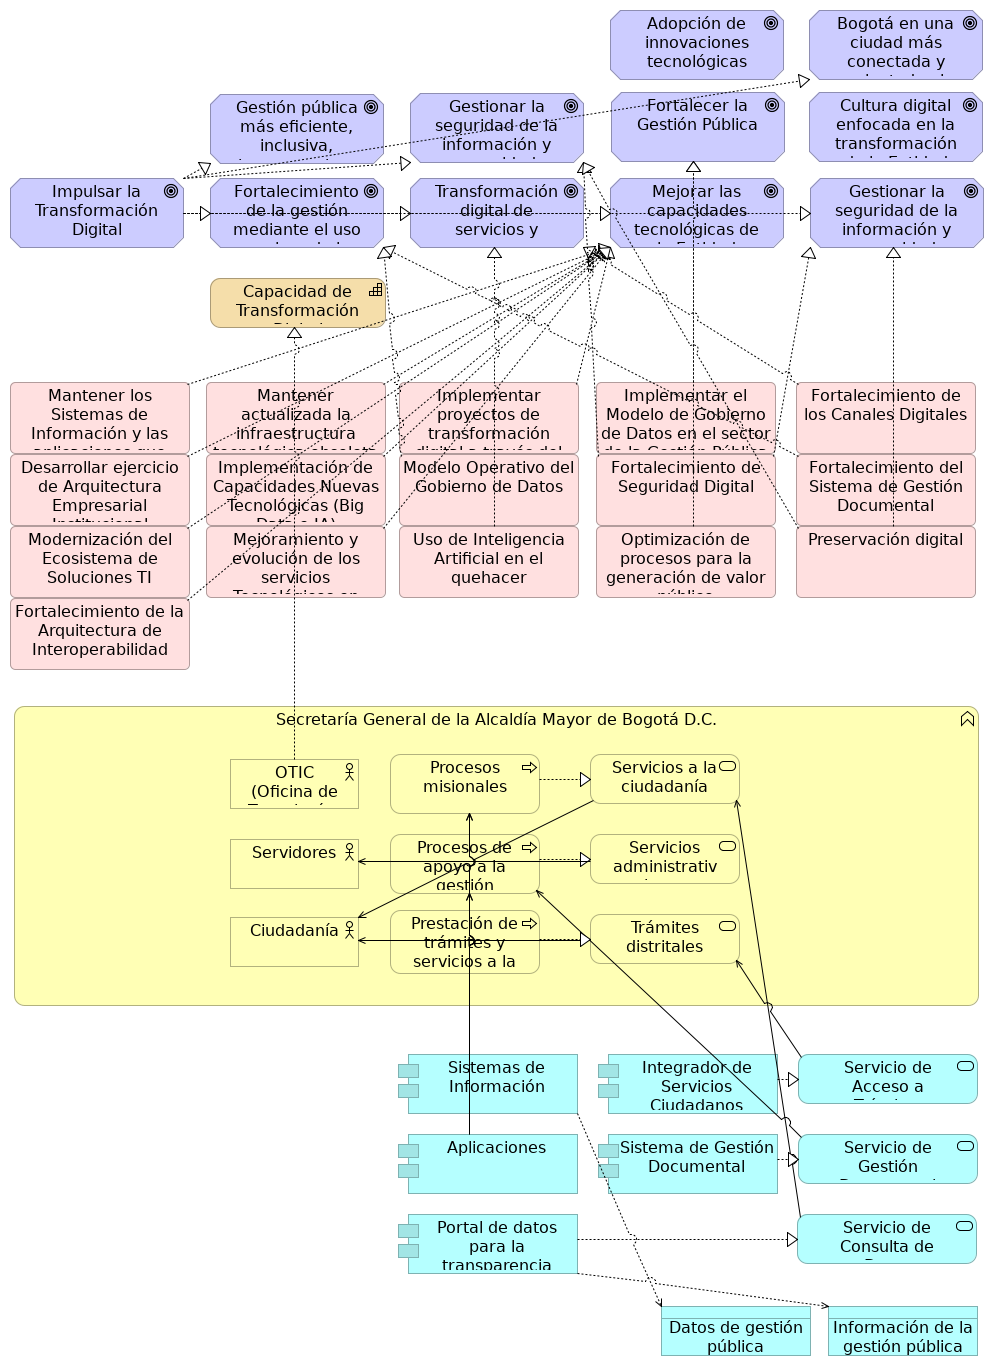
\includegraphics{images/06.BMM.ObjetivoseIniciativas.PETISG.png}
\caption{06.BMM. Objetivos e Iniciativas. PETI SG. \emph{Fuente:
Propuesta servicios de ingeniería y evaluación de arquitectura
Arquitectura de Aplicaciones Secretaria de la Alcaldía de Bogotá
(2025)}}\label{fig:id-710b67ee56954bd891264181bf9a408f}
\end{figure}

\subsubsection{Adopción de innovaciones tecnológicas para apoyar áreas
misionales
clave}\label{sec:adopciuxf3n-de-innovaciones-tecnoluxf3gicas-para-apoyar-uxe1reas-misionales-clave}

Objetivo de integrar nuevas tecnologías para mejorar funciones
principales. \#\#\# Bogotá en una ciudad más conectada y orientada al
bienestar de la ciudadanía Visión a largo plazo para la ciudad impulsada
por la digitalización. \#\#\# OETI03: Gestionar la seguridad de la
información y la seguridad digital Gestionar la seguridad de la
información y la seguridad digital mediante la adopción de políticas,
controles y campañas de concienciación que fomenten una cultura digital
segura, así como la implementación de estrategias para asegurar la
continuidad de los servicios de TIC. \#\#\# Fortalecer la Gestión
Pública Objetivo de TI de alto nivel optimizar (mejorar la eficiencia y
eficacia) los procesos y servicios de la administración pública.

\subsubsection{Cultura digital enfocada en la transformación de la
Entidad}\label{sec:cultura-digital-enfocada-en-la-transformaciuxf3n-de-la-entidad}

Meta de fomentar una mentalidad y habilidades digitales dentro de la
organización. \#\#\# Gestión pública más eficiente, inclusiva,
transparente y confiable Resultado deseado de una administración pública
mejorada para los ciudadanos. \#\#\# Impulsar la Transformación Digital
Meta principal del PETI, buscando modernizar la entidad a través de
tecnologías digitales. Contiene a la Política de Gobierno Digital.
\#\#\# Fortalecimiento de la gestión mediante el uso y mejora de las
tecnologías Objetivo de mejorar la gestión pública mediante la
aplicación de TI. \#\#\# Transformación digital de servicios y procesos
administrativos Meta de digitalizar y optimizar los servicios y procesos
internos y externos. \#\#\# Mejorar las capacidades tecnológicas de la
Entidad (objetivo estratégico de TI) Meta de TI para modernizar y
potenciar la infraestructura y habilidades tecnológicas. \#\#\#
Gestionar la seguridad de la información y seguridad digital (objetivo
estratégico de TI) Objetivo de TI para proteger los activos de
información y garantizar la ciberseguridad. \#\#\# Capacidad de
Transformación Digital Habilidad de la entidad para adaptarse y
evolucionar digitalmente. \#\#\# Mantener los Sistemas de Información y
las aplicaciones que apalanquen los procesos misionales y de apoyo a la
gestión Actividad continua para asegurar la operatividad y soporte de
los sistemas de información clave. \#\#\# Mantener actualizada la
infraestructura tecnológica obsoleta Proyecto recurrente para asegurar
la modernización y sostenibilidad de la infraestructura de TI. \#\#\#
Implementar proyectos de transformación digital a través del uso de
Tecnologías de Cuarta Revolución Industrial (4RI) Ejecución de
iniciativas que adoptan tecnologías avanzadas para la transformación
digital. \#\#\# Implementar el Modelo de Gobierno de Datos en el sector
de la Gestión Pública Proyecto para poner en práctica el marco de
gobernanza de datos en el ámbito público. \#\#\# Fortalecimiento de los
Canales Digitales Iniciativa para mejorar la calidad y alcance de los
canales de atención digitales. \#\#\# Desarrollar ejercicio de
Arquitectura Empresarial Institucional Proyecto para establecer y
madurar la práctica de Arquitectura Empresarial en la entidad. \#\#\#
Implementación de Capacidades Nuevas Tecnológicas (Big Data e IA)
Iniciativa para incorporar tecnologías emergentes de la Cuarta
Revolución Industrial para optimizar procesos, impulsar la innovación y
garantizar la transformación digital. \#\#\# Modelo Operativo del
Gobierno de Datos Proyecto para definir e implementar un marco de
gobernanza de datos. \#\#\# Fortalecimiento de Seguridad Digital
Iniciativa para proteger la infraestructura y los datos de amenazas
digitales. \#\#\# Fortalecimiento del Sistema de Gestión Documental
Iniciativa para el desarrollo e implementación de herramientas y
procesos avanzados para optimizar la clasificación, almacenamiento,
acceso y control de la documentación institucional. \#\#\# Modernización
del Ecosistema de Soluciones TI Proyecto para actualizar y optimizar el
conjunto de soluciones tecnológicas. \#\#\# Mejoramiento y evolución de
los servicios Tecnológicos en Nube Iniciativa para optimizar y expandir
el uso de servicios cloud. \#\#\# Uso de Inteligencia Artificial en el
quehacer Proyecto para integrar la IA en las operaciones diarias de la
entidad. \#\#\# Optimización de procesos para la generación de valor
público Proyecto para revisar y mejorar los procesos internos con foco
en el valor para el ciudadano. \#\#\# Preservación digital Proyecto para
asegurar la conservación y accesibilidad a largo plazo de los activos
digitales. \#\#\# Fortalecimiento de la Arquitectura de
Interoperabilidad Iniciativa para mejorar la comunicación e integración
entre sistemas y entidades. \#\#\# Secretaría General de la Alcaldía
Mayor de Bogotá D.C. Entidad principal de la administración distrital.
\#\#\# Procesos misionales Procesos clave que definen la razón de ser de
la entidad. \#\#\# Servicios a la ciudadanía Conjunto de servicios
ofrecidos a los ciudadanos. \#\#\# OTIC (Oficina de Tecnologías de la
Información y las Comunicaciones) Área encargada de la gestión de TI y
comunicaciones en la Secretaría General. \#\#\# Procesos de apoyo a la
gestión Procesos internos que facilitan la operación de la entidad.
\#\#\# Servicios administrativos internos Servicios de apoyo para el
funcionamiento interno de la entidad. \#\#\# Servidores Personal de la
entidad que participa en los procesos de negocio. \#\#\# Prestación de
trámites y servicios a la ciudadanía Proceso central para la interacción
con los ciudadanos. \#\#\# Trámites distritales Trámites específicos que
los ciudadanos pueden realizar. \#\#\# Ciudadanía Actores externos que
consumen los servicios de la Alcaldía. \#\#\# Sistemas de Información
Conjunto genérico de sistemas que soportan las operaciones de la
entidad. \#\#\# Integrador de Servicios Ciudadanos Plataforma unificada
para acceder a diversos servicios y trámites ciudadanos. \#\#\# Servicio
de Acceso a Trámites Servicio que permite a los ciudadanos iniciar y
gestionar trámites en línea. \#\#\# Aplicaciones Software específico
utilizado para diversas funciones de negocio. \#\#\# Sistema de Gestión
Documental Sistema para la administración y control de documentos
digitales. \#\#\# Servicio de Gestión Documental Servicio para la
creación, almacenamiento y recuperación de documentos. \#\#\# Portal de
datos para la transparencia Plataforma que facilita el acceso público a
datos e información gubernamental. \#\#\# Servicio de Consulta de Datos
Servicio provisto por el portal de datos para acceder a información
pública. \#\#\# Datos de gestión pública Información general utilizada
en los procesos de la administración pública. \#\#\# Información de la
gestión pública Conjunto de datos e información relevante para la
transparencia y la toma de decisiones.

\subsection{Iniciativas}\label{sec:iniciativas}

\begin{quote}
\end{quote}

El modelo de diagrama ArchiMate denominado ``06.Estrategia.
Iniciativas'' se posiciona como un componente clave para visualizar y
comunicar la transformación estratégica de la organización. Su propósito
central es ilustrar cómo los objetivos de alto nivel se desglosan en
planes de acción concretos o ``iniciativas'', conectando así la visión
estratégica con la ejecución. Este tipo de diagrama es fundamental para
alinear los esfuerzos y las inversiones empresariales, asegurando que
cada proyecto y programa contribuya directamente a la consecución de las
metas corporativas.

Un modelo de ``Estrategia. Iniciativas'' bien estructurado es un activo
invaluable para la gestión del portafolio de proyectos, la toma de
decisiones informadas sobre la asignación de recursos y la comunicación
efectiva de la hoja de ruta estratégica a todos los niveles de la
empresa, impulsando la coherencia y el éxito en la implementación.

\begin{figure}
\centering
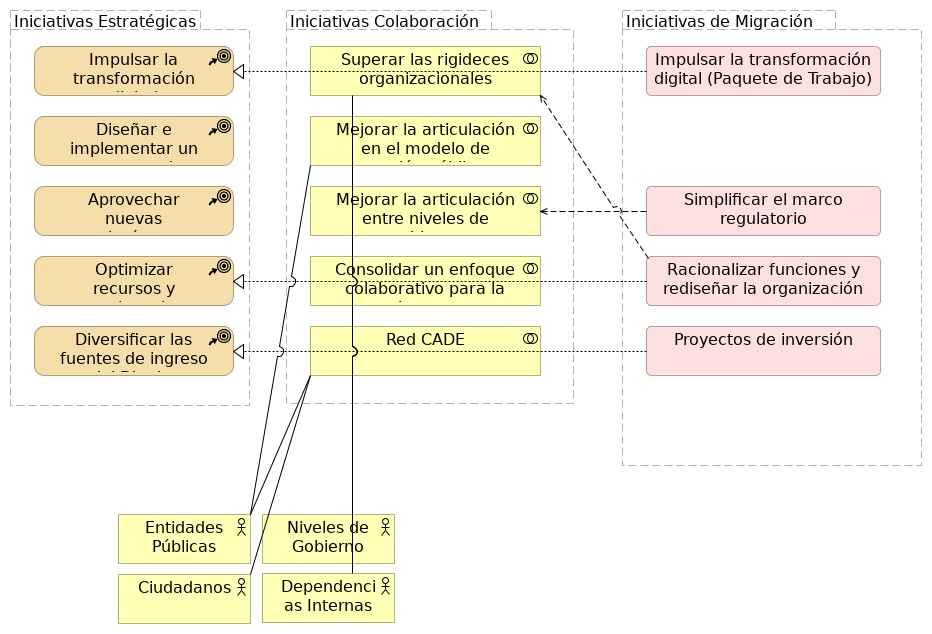
\includegraphics{images/06.Estrategia.Iniciativas.png}
\caption{06.Estrategia. Iniciativas. \emph{Fuente: Propuesta servicios
de ingeniería y evaluación de arquitectura Arquitectura de Aplicaciones
Secretaria de la Alcaldía de Bogotá
(2025)}}\label{fig:id-cc506af7ae2e4eadbe0ef317bcdce54d}
\end{figure}

\subsubsection{Iniciativas
Estratégicas}\label{sec:iniciativas-estratuxe9gicas}

\subsubsection{Impulsar la transformación
digital}\label{sec:impulsar-la-transformaciuxf3n-digital-1}

Enfoque estratégico para la modernización de los procesos y servicios
mediante tecnologías digitales. \#\#\# Diseñar e implementar un esquema
de gobernanza de territorio inteligente Define las directrices y
estructuras para la gestión de un ecosistema urbano inteligente. \#\#\#
Aprovechar nuevas tecnologías como la Inteligencia Artificial Estrategia
para integrar y explotar tecnologías emergentes en beneficio de la
gestión pública. \#\#\# Optimizar recursos y mejorar la operación
Enfoque para maximizar la eficiencia en el uso de los recursos
disponibles y mejorar el rendimiento operativo. \#\#\# Diversificar las
fuentes de ingreso del Distrito Estrategia para explorar y desarrollar
nuevas vías de financiación para el Distrito. \#\#\# Iniciativas
Colaboración

\subsubsection{Superar las rigideces
organizacionales}\label{sec:superar-las-rigideces-organizacionales}

Colaboración orientada a eliminar barreras estructurales que impiden la
agilidad y eficiencia de la entidad. \#\#\# Mejorar la articulación en
el modelo de gestión pública Colaboración para integrar y coordinar
mejor las diferentes áreas y procesos de la gestión pública. \#\#\#
Mejorar la articulación entre niveles de gobierno Colaboración enfocada
en una mayor coordinación y cooperación entre los distintos niveles de
la administración pública. \#\#\# Consolidar un enfoque colaborativo
para la gobernanza metropolitana Colaboración para establecer una visión
y gestión unificada de los asuntos metropolitanos. \#\#\# Red CADE Red
de colaboración entre entidades para la prestación de servicios de
atención presencial a ciudadanos. \#\#\# Iniciativas de Migración

\subsubsection{Impulsar la transformación digital (Paquete de
Trabajo)}\label{sec:impulsar-la-transformaciuxf3n-digital-paquete-de-trabajo}

Conjunto de actividades para iniciar y desarrollar la transformación
digital de la entidad. \#\#\# Simplificar el marco regulatorio Paquete
de trabajo enfocado en la revisión y simplificación de las normativas
vigentes. \#\#\# Racionalizar funciones y rediseñar la organización
Paquete de trabajo para optimizar la estructura funcional y
organizacional de la entidad. \#\#\# Proyectos de inversión Paquete de
trabajo general que engloba todas las iniciativas de inversión para
mejoras. \#\#\# Entidades Públicas Actores organizacionales que
participan en las colaboraciones y ofrecen servicios. \#\#\# Niveles de
Gobierno Diferentes estamentos gubernamentales (nacional, distrital,
local) que requieren articulación. \#\#\# Dependencias Internas Unidades
organizacionales internas de la Secretaría General o la Alcaldía Mayor.
\#\#\# Ciudadanos Beneficiarios finales de los servicios y actores
involucrados en la interacción con la administración.

\subsection{Necesidades y
Aplicaciones}\label{sec:necesidades-y-aplicaciones}

\begin{quote}
\end{quote}

\begin{figure}
\centering
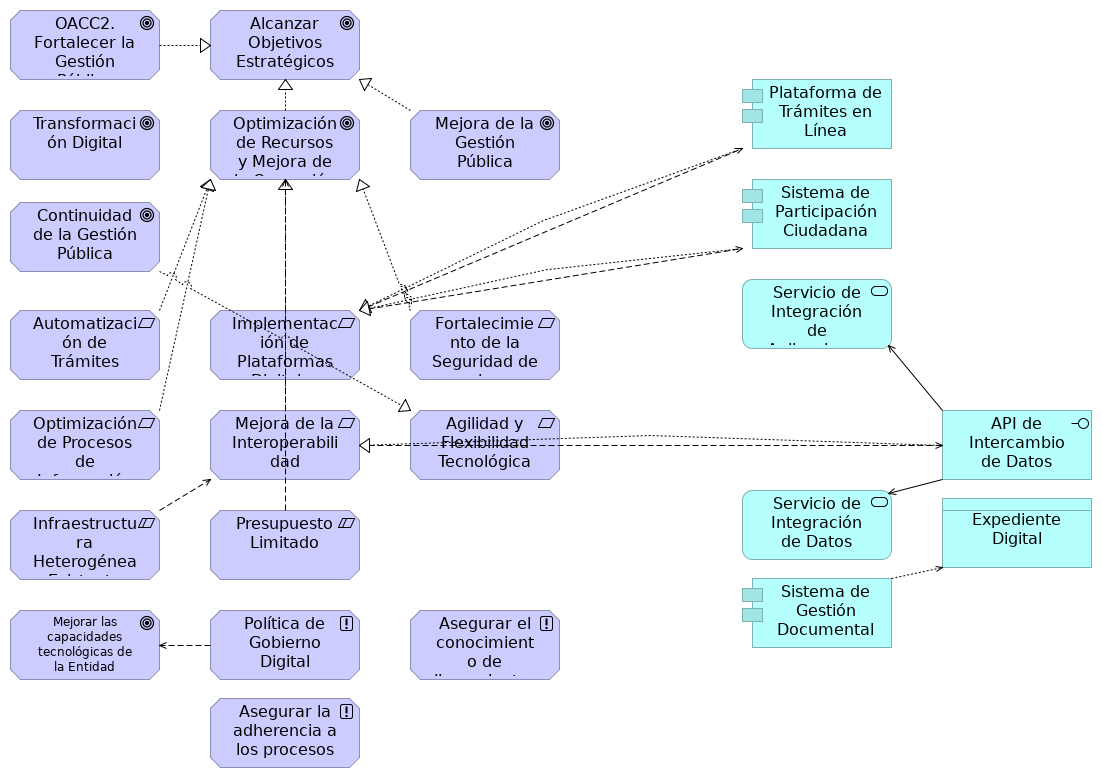
\includegraphics{images/06.Negocio.n1.a.NecesidadesyAplicaciones.png}
\caption{06.Negocio.n1.a. Necesidades y Aplicaciones. \emph{Fuente:
Propuesta servicios de ingeniería y evaluación de arquitectura
Arquitectura de Aplicaciones Secretaria de la Alcaldía de Bogotá
(2025)}}\label{fig:id-73084877ba5b4f859a7aa197be93b750}
\end{figure}

\subsubsection{Fortalecer la Gestión
Pública}\label{sec:fortalecer-la-gestiuxf3n-puxfablica-1}

Objetivo de TI de alto nivel optimizar (mejorar la eficiencia y
eficacia) los procesos y servicios de la administración pública.

\subsubsection{Alcanzar Objetivos
Estratégicos}\label{sec:alcanzar-objetivos-estratuxe9gicos}

Meta general de la Secretaría General para cumplir con su misión y
visión. \#\#\# Plataforma de Trámites en Línea Componente de aplicación
que permite la realización de trámites digitales. \#\#\# Transformación
Digital Objetivo clave relacionado con la modernización y digitalización
de los servicios y operaciones.

La transformación digital es un motor fundamental para alinear las
estrategias, procesos y tecnologías de la Secretaría General. Esta
transformación busca:

\begin{itemize}
\tightlist
\item
  Cerrar las brechas en la Política de Gobierno Digital, de la cual la
  Arquitectura Empresarial es un habilitador clave.
\item
  Modernizar la infraestructura tecnológica obsoleta para asegurar su
  continuidad y disponibilidad.
\item
  Integrar plataformas y ecosistemas digitales y superar la falta de
  interoperabilidad.
\item
  Automatizar trámites y estandarizar la gestión y gobernanza de datos
  públicos.
\item
  Adquirir software especializado en análisis de datos para mejorar la
  toma de decisiones basada en evidencia.
\item
  Generar análisis predictivos y prospectivos de resultados de gestión,
  que son insumos para la toma de decisiones.
\item
  Aprovechar nuevas tecnologías como la Inteligencia Artificial para
  mejorar los procesos y la relación con la ciudadanía.
\item
  Fortalecer la ciberseguridad y seguridad de la información para
  proteger la integridad, disponibilidad y confidencialidad de los datos
  y prevenir ataques.
\item
  La disponibilidad de personal adecuado para actualizar plataformas
  tecnológicas es una necesidad identificada para este eje, y los altos
  costos de la tecnología representan una limitación. \#\#\#
  Optimización de Recursos y Mejora de la Operación Objetivo de mejorar
  la eficiencia en el uso de los recursos y la calidad de las
  operaciones internas. \#\#\# Mejora de la Gestión Pública Objetivo
  general de elevar la calidad y el impacto de la gestión gubernamental.
  \#\#\# Sistema de Participación Ciudadana Componente de aplicación
  para facilitar la interacción y el feedback de los ciudadanos. \#\#\#
  Continuidad de la Gestión Pública Objetivo de asegurar que los
  programas y proyectos perduren entre diferentes administraciones.
  \#\#\# Servicio de Integración de Aplicaciones Servicio de aplicación
  para la unificación y el intercambio de funcionalidades. \#\#\#
  Automatización de Trámites Necesidad de digitalizar y automatizar los
  procesos de interacción con los ciudadanos. \#\#\# Implementación de
  Plataformas Digitales Requisito para desarrollar o adquirir sistemas
  para trámites y participación ciudadana. \#\#\# Fortalecimiento de la
  Seguridad de la Información Necesidad de proteger los datos y sistemas
  contra amenazas y vulnerabilidades. \#\#\# Optimización de Procesos de
  Información Requisito para mejorar la eficiencia y calidad en el
  manejo de la información. \#\#\# Mejora de la Interoperabilidad
  Necesidad de asegurar la comunicación y el intercambio de datos entre
  diferentes sistemas. \#\#\# Agilidad y Flexibilidad Tecnológica
  Requisito para que las soluciones tecnológicas puedan adaptarse
  rápidamente a nuevos cambios. \#\#\# API de Intercambio de Datos
  Interfaz de aplicación para permitir la comunicación entre diferentes
  sistemas. \#\#\# Servicio de Integración de Datos Servicio de
  aplicación para la unificación y el intercambio de información. \#\#\#
  Expediente Digital Objeto de datos en la capa de aplicación que
  representa un expediente electrónico. \#\#\# Infraestructura
  Heterogénea Existente Restricción derivada de la diversidad de
  sistemas y tecnologías ya implementadas. \#\#\# Presupuesto Limitado
  Restricción financiera para la ejecución de iniciativas y proyectos.
  \#\#\# Sistema de Gestión Documental Componente de aplicación para la
  gestión electrónica de documentos. \#\#\# Mejorar las capacidades
  tecnológicas de la Entidad (objetivo estratégico de TI) Meta de TI
  para modernizar y potenciar la infraestructura y habilidades
  tecnológicas. \#\#\# Política de Gobierno Digital Principios que
  guiarán el diseño y la evolución de la arquitectura de solución. Son
  declaraciones de intención de la SG que deben ser cumplidas. \#\#\#
  Asegurar el conocimiento de lineamientos y directrices Principios de
  gobernanza interna. \#\#\# Asegurar la adherencia a los procesos y
  procedimientos establecidos Principios de gobernanza interna.
\end{itemize}

\subsection{Preocupaciones
(debilidades)}\label{sec:preocupaciones-debilidades}

\begin{quote}
\end{quote}

\begin{figure}
\centering
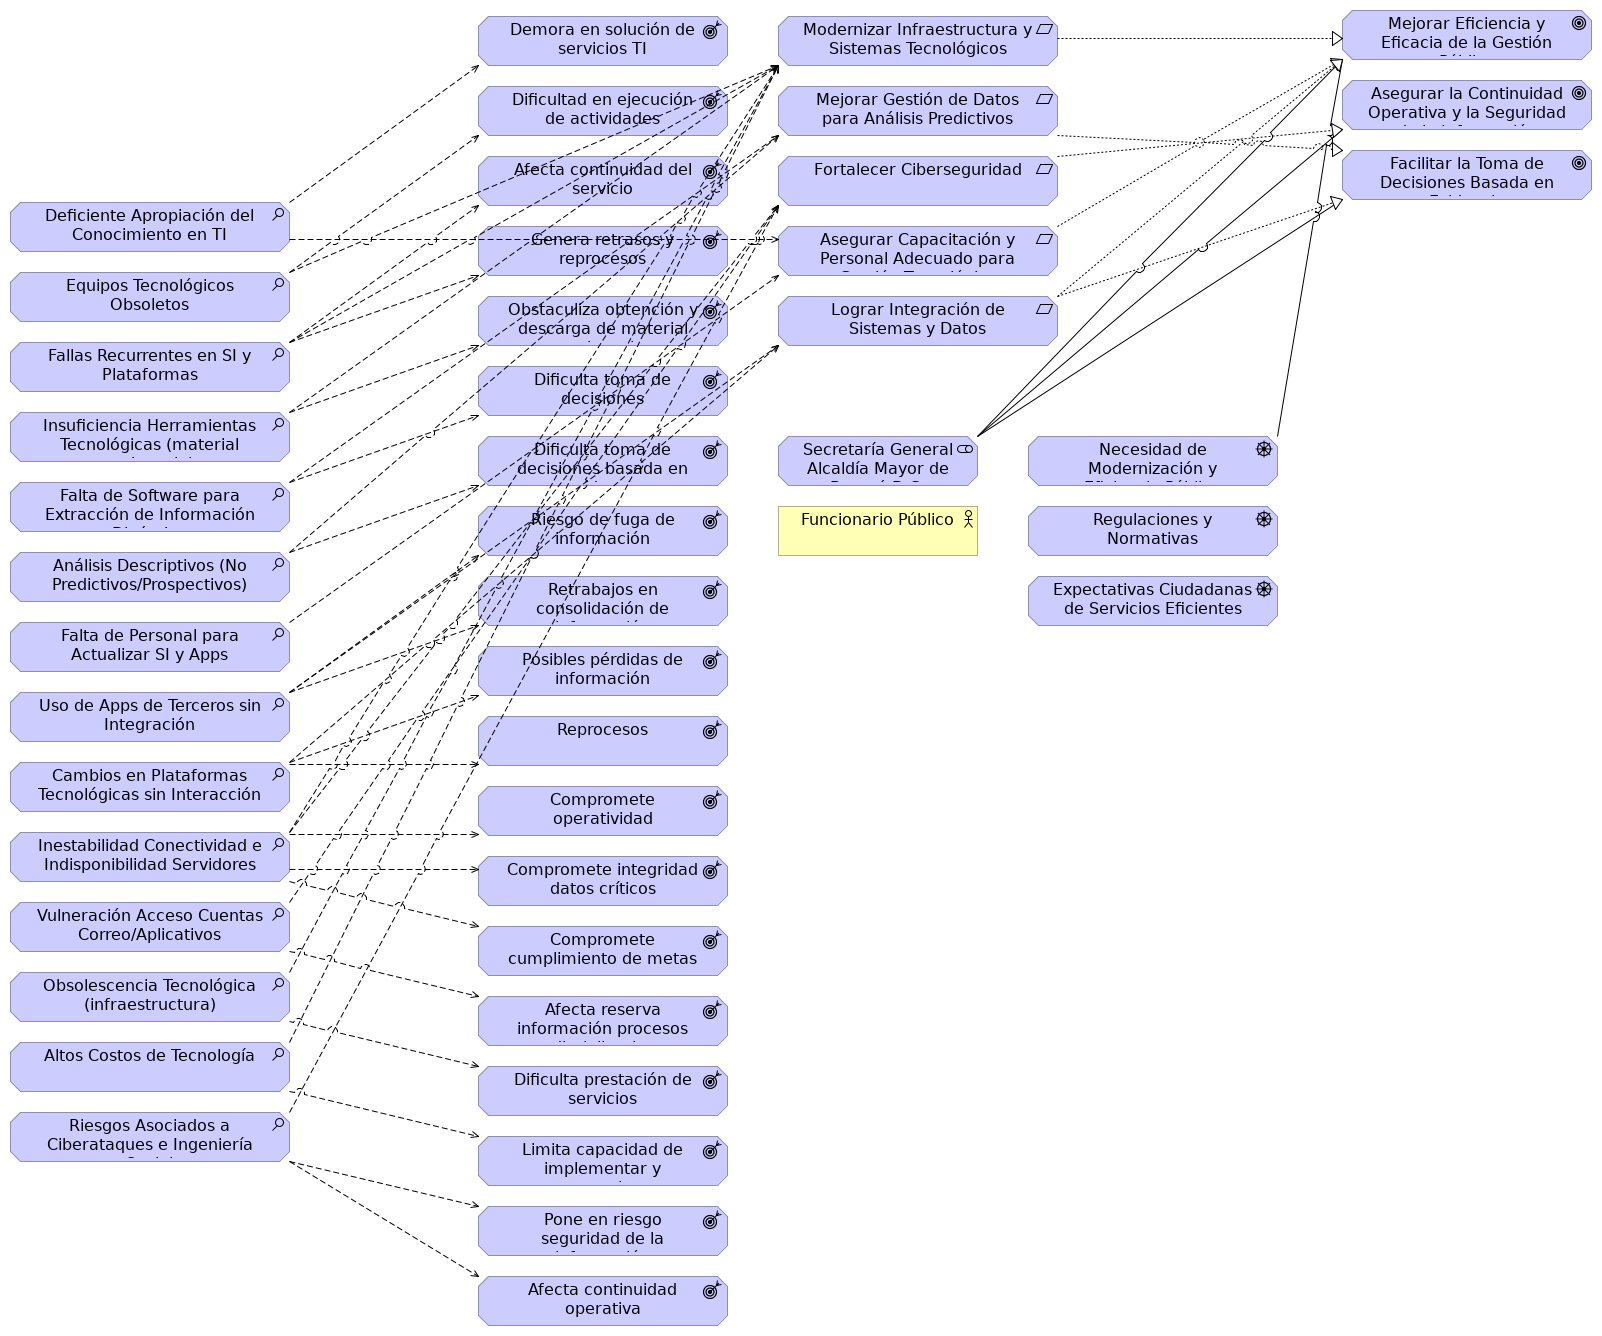
\includegraphics{images/06.Negocio.n3.Preocupaciones(debilidades).png}
\caption{06.Negocio.n3. Preocupaciones (debilidades). \emph{Fuente:
Propuesta servicios de ingeniería y evaluación de arquitectura
Arquitectura de Aplicaciones Secretaria de la Alcaldía de Bogotá
(2025)}}\label{fig:id-8c74f3e0c66d4a509f2af637eae4a268}
\end{figure}

\subsubsection{Mejorar Eficiencia y Eficacia de la Gestión
Pública}\label{sec:mejorar-eficiencia-y-eficacia-de-la-gestiuxf3n-puxfablica}

Meta estratégica para optimizar la gestión de la entidad.. \#\#\# Demora
en solución de servicios TI Impacto de la deficiente apropiación del
conocimiento en TI. \#\#\# Modernizar Infraestructura y Sistemas
Tecnológicos Requisito para actualizar los componentes tecnológicos de
la entidad. \#\#\# Asegurar la Continuidad Operativa y la Seguridad de
la Información Meta estratégica para garantizar la operación
ininterrumpida y la protección de datos. \#\#\# Dificultad en ejecución
de actividades Impacto de los equipos tecnológicos obsoletos. \#\#\#
Mejorar Gestión de Datos para Análisis Predictivos Requisito para
implementar capacidades de análisis de datos avanzados. \#\#\# Facilitar
la Toma de Decisiones Basada en Evidencia Meta estratégica para mejorar
los procesos de decisión mediante el uso de datos y análisis. \#\#\#
Afecta continuidad del servicio Impacto de fallas recurrentes en SI y
plataformas. \#\#\# Fortalecer Ciberseguridad Requisito para implementar
medidas de protección contra amenazas cibernéticas. \#\#\# Deficiente
Apropiación del Conocimiento en TI Debilidad interna relacionada con la
gestión y el uso del conocimiento en tecnologías de la información.
\#\#\# Genera retrasos y reprocesos Impacto de fallas recurrentes en SI
y plataformas. \#\#\# Asegurar Capacitación y Personal Adecuado para
Gestión Tecnológica Requisito para garantizar el talento humano
necesario para la gestión de TI. \#\#\# Equipos Tecnológicos Obsoletos
Debilidad de infraestructura que afecta la ejecución de actividades.
\#\#\# Obstaculiza obtención y descarga de material probatorio Impacto
de la insuficiencia de herramientas tecnológicas para material
probatorio. \#\#\# Lograr Integración de Sistemas y Datos Requisito para
eliminar silos de información y permitir el flujo de datos entre
sistemas. \#\#\# Fallas Recurrentes en SI y Plataformas Debilidad en la
estabilidad y confiabilidad de los sistemas de información. \#\#\#
Dificulta toma de decisiones Impacto de la falta de software para
extracción de información dinámica. \#\#\# Insuficiencia Herramientas
Tecnológicas (material probatorio) Debilidad en la capacidad de las
herramientas para soportar procesos críticos. \#\#\# Dificulta toma de
decisiones basada en evidencia Impacto de los análisis descriptivos, no
predictivos/prospectivos. \#\#\# Secretaría General Alcaldía Mayor de
Bogotá D.C. La entidad principal interesada en la mejora de la
arquitectura tecnológica. \#\#\# Necesidad de Modernización y Eficiencia
Pública Factor impulsor que motiva la transformación y mejora
tecnológica. \#\#\# Falta de Software para Extracción de Información
Dinámica Debilidad en la capacidad de análisis y reporte de información
para la toma de decisiones. \#\#\# Riesgo de fuga de información Impacto
del uso de Apps de terceros sin integración. \#\#\# Funcionario Público
El usuario final y actor de negocio afectado por las debilidades
tecnológicas. \#\#\# Regulaciones y Normativas Factores externos que
impulsan el cumplimiento y la adaptación tecnológica. \#\#\# Análisis
Descriptivos (No Predictivos/Prospectivos) Debilidad en la capacidad de
la entidad para realizar análisis avanzados que apoyen la toma de
decisiones basada en evidencia. \#\#\# Retrabajos en consolidación de
información Impacto del uso de Apps de terceros sin integración. \#\#\#
Expectativas Ciudadanas de Servicios Eficientes Factor externo
relacionado con la demanda de servicios públicos ágiles y efectivos.
\#\#\# Falta de Personal para Actualizar SI y Apps Debilidad en la
disponibilidad de recursos humanos para el mantenimiento y evolución de
sistemas. \#\#\# Posibles pérdidas de información Impacto de cambios en
plataformas tecnológicas sin interacción. \#\#\# Uso de Apps de Terceros
sin Integración Debilidad en la arquitectura de integración, generando
riesgos y reprocesos. \#\#\# Reprocesos Impacto de cambios en
plataformas tecnológicas sin interacción. \#\#\# Cambios en Plataformas
Tecnológicas sin Interacción Debilidad en la gestión del cambio
tecnológico y la interoperabilidad. \#\#\# Compromete operatividad
Impacto de inestabilidad de conectividad e indisponibilidad de
servidores. \#\#\# Inestabilidad Conectividad e Indisponibilidad
Servidores Debilidad en la infraestructura de red y servidores,
afectando la continuidad operativa. \#\#\# Compromete integridad datos
críticos Impacto de inestabilidad de conectividad e indisponibilidad de
servidores. \#\#\# Vulneración Acceso Cuentas Correo/Aplicativos
Debilidad en la seguridad de acceso, comprometiendo la confidencialidad
de la información. \#\#\# Compromete cumplimiento de metas Impacto de
inestabilidad de conectividad e indisponibilidad de servidores. \#\#\#
Obsolescencia Tecnológica (infraestructura) Debilidad general de la
infraestructura tecnológica que requiere renovación. \#\#\# Afecta
reserva información procesos disciplinarios Impacto de la vulneración de
acceso a cuentas correo/aplicativos. \#\#\# Altos Costos de Tecnología
Debilidad financiera que limita la inversión en tecnología avanzada.
\#\#\# Dificulta prestación de servicios Impacto de la obsolescencia
tecnológica de la infraestructura. \#\#\# Riesgos Asociados a
Ciberataques e Ingeniería Social Debilidad en la postura de seguridad
frente a amenazas externas. \#\#\# Limita capacidad de implementar y
mantener sistemas eficientes Impacto de los altos costos de la
tecnología. \#\#\# Pone en riesgo seguridad de la información Impacto de
riesgos asociados a ciberataques e ingeniería social. \#\#\# Afecta
continuidad operativa Impacto de riesgos asociados a ciberataques e
ingeniería social.

\subsection{Oportunidades}\label{sec:oportunidades}

\begin{quote}
\end{quote}

Esta vista general presenta las relaciones clave entre las oportunidades
(drivers), las metas, las capacidades estratégicas, los cursos de
acción, los flujos de valor y los resultados, ofreciendo una perspectiva
integral de la transformación propuesta.
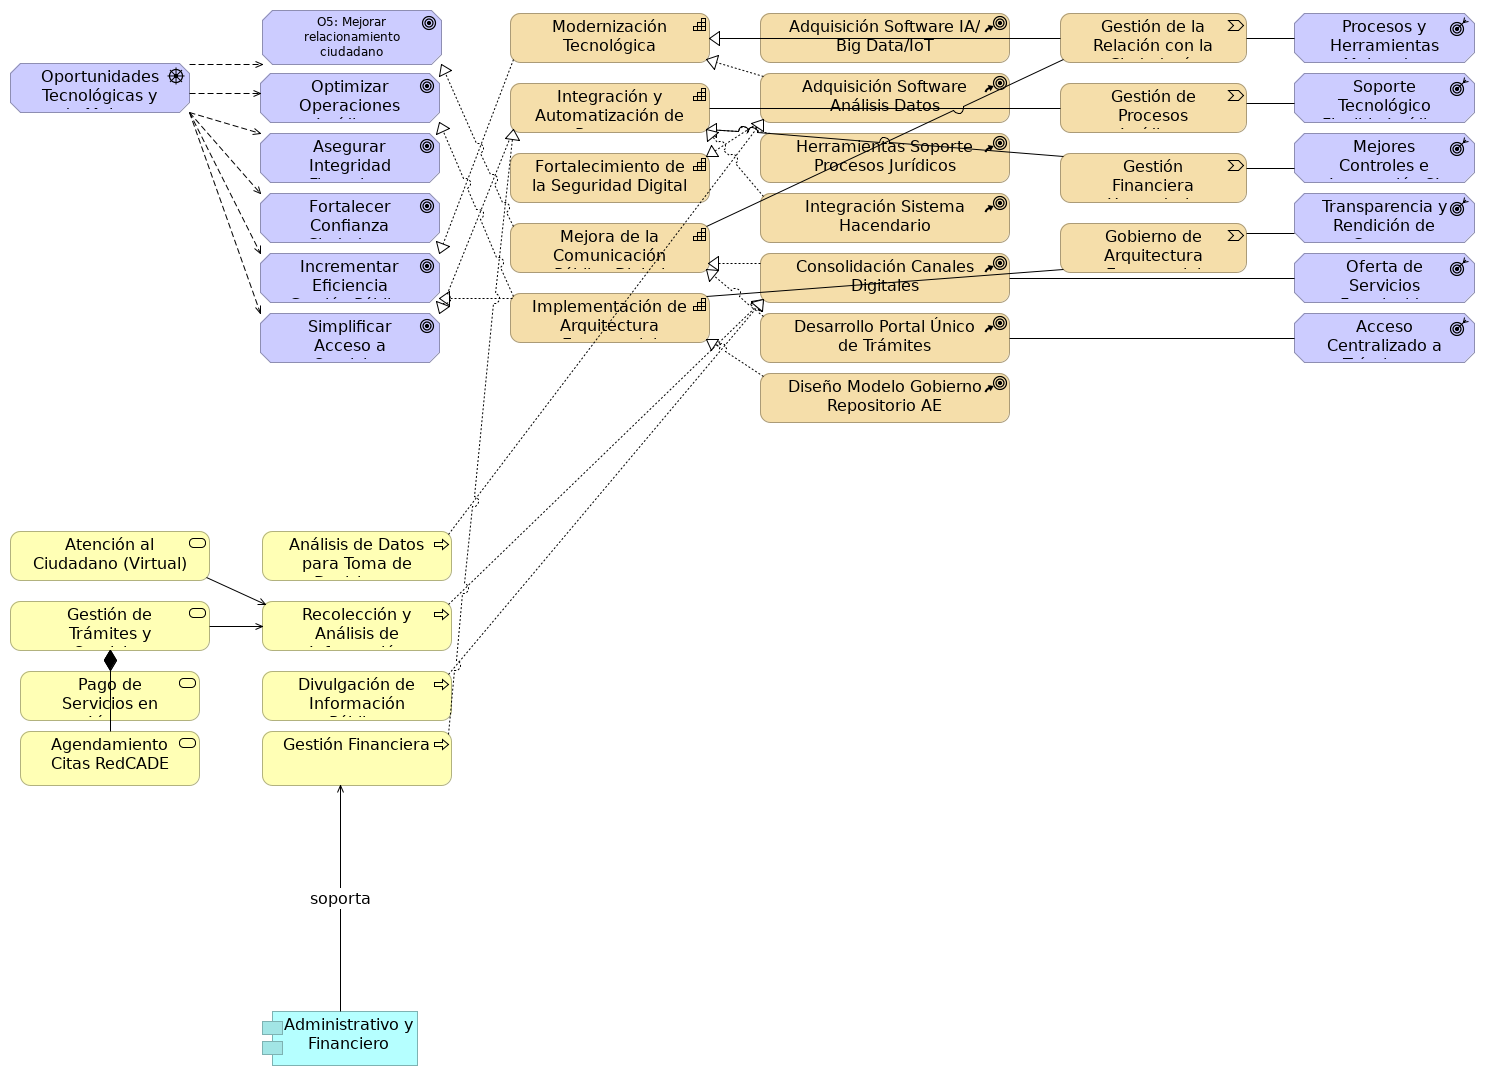
\includegraphics{images/06.Negocio.n4.Oportunidades.png}

\subsubsection{O5: Mejorar relacionamiento
ciudadano}\label{sec:o5-mejorar-relacionamiento-ciudadano}

Mejorar el relacionamiento de la ciudadanía con el gobierno distrital a
través del fortalecimiento de la oferta institucional, la modernización
de los canales de atención y la cualificación del talento humano,
contribuyendo al aumento de la confianza y satisfacción ciudadana.
\#\#\# Modernización Tecnológica Capacidad de incorporar nuevas
tecnologías como IA, Big Data e IoT para mejorar procesos y
herramientas. \#\#\# Adquisición Software IA/Big Data/IoT Iniciativa
para adquirir software especializado que soporte la modernización
tecnológica. \#\#\# Gestión de la Relación con la Ciudadanía Flujo de
valor que abarca todas las interacciones y servicios ofrecidos a los
ciudadanos. \#\#\# Procesos y Herramientas Mejorados Resultado esperado
de la modernización tecnológica y la implementación de IA. \#\#\#
Oportunidades Tecnológicas y de Mejora Impulsor principal derivado del
análisis de las oportunidades para la transformación digital y la
eficiencia en la gestión pública. \#\#\# Optimizar Operaciones Jurídicas
Meta de mejorar la eficiencia y el soporte tecnológico de los procesos
jurídicos. \#\#\# Adquisición Software Análisis Datos Iniciativa para
adquirir software que permita el análisis de datos para la toma de
decisiones. \#\#\# Soporte Tecnológico Flexible Jurídico Resultado de
contar con herramientas tecnológicas que se adapten a las operaciones
jurídicas. \#\#\# Integración y Automatización de Procesos Capacidad
para unificar y optimizar flujos de trabajo mediante herramientas
tecnológicas. \#\#\# Gestión de Procesos Jurídicos Flujo de valor
relacionado con la gestión y soporte de las operaciones jurídicas.
\#\#\# Asegurar Integridad Financiera Meta de fortalecer los controles y
la integración con el sistema hacendario. \#\#\# Herramientas Soporte
Procesos Jurídicos Iniciativa para implementar herramientas tecnológicas
para el soporte y evaluación de procesos jurídicos. \#\#\# Mejores
Controles e Integración SI Resultado de la integración de sistemas de
información con el Sistema Hacendario. \#\#\# Fortalecimiento de la
Seguridad Digital Capacidad de proteger los activos digitales y la
información sensible de la entidad. \#\#\# Gestión Financiera Hacendaria
Flujo de valor que involucra los sistemas y procesos financieros y
hacendarios. \#\#\# Fortalecer Confianza Ciudadana Meta de aumentar la
confianza pública a través de la transparencia y seguridad digital.
\#\#\# Integración Sistema Hacendario Iniciativa para mejorar los
controles e integración de los sistemas de información con el Sistema
Hacendario. \#\#\# Transparencia y Rendición de Cuentas Aumentada
Resultado de la estandarización de procesos y sistemas de información
gracias a la AE. \#\#\# Mejora de la Comunicación Pública Digital
Capacidad de interactuar y proveer información a los ciudadanos de forma
efectiva a través de medios digitales. \#\#\# Gobierno de Arquitectura
Empresarial Flujo de valor que establece los lineamientos y procesos
para la gobernanza de la arquitectura empresarial. \#\#\# Incrementar
Eficiencia Gestión Pública Meta de optimizar los procesos internos y la
prestación de servicios gubernamentales. \#\#\# Consolidación Canales
Digitales Iniciativa para consolidar herramientas y canales digitales
para fortalecer la oferta y celeridad de servicios. \#\#\# Oferta de
Servicios Fortalecida Resultado de la consolidación de canales e
información para una mejor oferta de servicios. \#\#\# Implementación de
Arquitectura Empresarial Capacidad de establecer y gestionar la
disciplina de arquitectura empresarial para guiar la transformación
digital. \#\#\# Simplificar Acceso a Servicios Meta de hacer más
accesibles y eficientes los trámites y servicios digitales para la
ciudadanía. \#\#\# Desarrollo Portal Único de Trámites Iniciativa para
unificar la oferta de trámites y servicios en un portal digital
centralizado. \#\#\# Acceso Centralizado a Trámites y Servicios
Resultado de la unificación de trámites y servicios en un portal único.
\#\#\# Diseño Modelo Gobierno Repositorio AE Iniciativa para crear un
modelo de gobernanza para el Repositorio de Arquitectura Empresarial.
\#\#\# Atención al Ciudadano (Virtual) Servicio de negocio para la
atención a través de canales virtuales como SuperCADE Virtual, chat,
chat-Bot y videollamadas. \#\#\# Análisis de Datos para Toma de
Decisiones Proceso de negocio que utiliza software especializado para el
análisis de datos. \#\#\# Gestión de Trámites y Servicios Servicio de
negocio que permite el acceso y realización de trámites y servicios
públicos. \#\#\# Recolección y Análisis de Información Proceso de
negocio enfocado en la automatización de la recolección y análisis de
datos. \#\#\# Pago de Servicios en Línea Sub-servicio de negocio que
permite realizar pagos no tributarios en línea. \#\#\# Divulgación de
Información Pública Proceso de negocio para la difusión optimizada de
información a través de sistemas digitales. \#\#\# Agendamiento Citas
RedCADE Sub-servicio de negocio que facilita la programación de citas en
la RedCADE desde
casa.\sidenote{This is a sidenote. This template features a large margin specifically so you can put notes, figures, tables and other things into it as additional material to the main content in the text block.}

Donec in elit ac ante vestibulum rhoncus. Pellentesque ligula tortor, aliquet malesuada nulla tristique vitae. Aliquam mi sem, varius eu pellentesque et, tristique nec quam. Vestibulum pellentesque in dui et venenatis. Sed malesuada elit pellentesque sapien aliquet porta. In at facilisis diam. Duis id ante tellus.\sidenote[][2cm]{This sidenote has been pushed down the page manually with an optional parameter, otherwise it would be right under the one above.} % This first optional argument to a sidenote is the symbol to use (leave this empty for automatic numbering) and the second is the vertical offset (positive is down, negative is up)

In diam libero, vulputate quis accumsan non, auctor in ipsum. Praesent cursus velit eget lacus sodales porta. Proin quis risus ut velit euismod scelerisque ut sed neque. Cras sagittis, dolor ac ullamcorper auctor, tortor dui facilisis diam, at sagittis nisi ipsum a neque. Nullam vel mattis nisi. Ut interdum ut diam at ornare. Nulla ultrices elit justo, vitae tristique massa vulputate sit amet.

\nonumsidenote{
	}Vestibulum erat felis, cursus vitae convallis ac, commodo eu nisi. Nulla facilisi. Mauris dignissim nisi felis, a mollis ex accumsan vel. Suspendisse bibendum vitae nibh in suscipit. Vestibulum et finibus eros. Nulla facilisi. Cras luctus aliquam finibus. In nec justo nec orci malesuada faucibus.

\subsubsection{Subsubsection Title} % Third level section

\begin{fullwidth} % Use the whole page width
	\textit{This is an example of a full width paragraph\ldots} Curabitur id placerat orci. Vivamus pulvinar augue ac feugiat blandit. Donec in ultricies mi. Nam eu lacus ac augue aliquet consectetur. Praesent dui risus, sollicitudin nec felis ut, posuere ultricies dolor. Sed massa nulla, dignissim eget sem sit amet, eleifend fermentum dui. Phasellus consequat sem vel turpis finibus, a aliquam risus malesuada.
\end{fullwidth}

Maecenas consectetur metus at tellus finibus condimentum. Proin arcu lectus, ultrices non tincidunt et, tincidunt ut quam. Integer luctus posuere est, non maximus ante dignissim quis. Nunc a cursus erat. Curabitur suscipit nibh in tincidunt sagittis. Nam malesuada vestibulum quam id gravida. Proin ut dapibus velit. Vestibulum eget quam quis ipsum semper convallis. Duis consectetur nibh ac diam dignissim, id condimentum enim dictum. Nam aliquet ligula eu magna pellentesque, nec sagittis leo lobortis. Aenean tincidunt dignissim egestas. Morbi efficitur risus ante, id tincidunt odio pulvinar vitae.

\paragraph{Paragraph Title} % Fourth level section

Lorem ipsum dolor sit amet, consectetur adipiscing elit. Aliquam auctor mi risus, quis tempor libero hendrerit at. Duis hendrerit placerat quam et semper. Nam ultricies metus vehicula arcu viverra, vel ullamcorper justo elementum. Pellentesque vel mi ac lectus cursus posuere et nec ex.

The section titles below show how multi-line section titles look at the 3 top levels.


%----------------------------------------------------------------------------------------
%	QUOTATIONS
%----------------------------------------------------------------------------------------

\section{Quotations}

Proin mollis urna posuere fringilla. Curabitur finibus, neque vitae vestibulum vestibulum, dolor sapien tincidunt augue, vel porta mauris metus nec mauris. Integer erat magna, porta id erat sed, lacinia volutpat erat. Nulla fermentum tellus arcu, eu iaculis ipsum malesuada aliquam. Duis et lacus maximus, consectetur metus et, eleifend arcu. Vestibulum condimentum diam vitae diam tincidunt viverra.\sidenotequote[-1cm]{\textbf{\LARGE ``}Lorem ipsum dolor sit amet, consectetur adipiscing elit. Praesent porttitor arcu luctus, imperdiet urna iaculis, mattis eros. Pellentesque iaculis odio vel nisl ullamcorper, nec faucibus ipsum molestie.\textbf{''}\\[4pt]\hfill--- John Smith, 1972} % Example margin quotation using the \sidenotequote custom command

\begin{quote}
	\textbf{\LARGE ``}Lorem ipsum dolor sit amet, consectetur adipiscing elit. Praesent porttitor arcu luctus, imperdiet urna iaculis, mattis eros. Pellentesque iaculis odio vel nisl ullamcorper, nec faucibus ipsum molestie. Sed dictum nisl non aliquet porttitor. Etiam vulputate arcu dignissim, finibus sem et, viverra nisl. Aenean luctus congue massa, ut laoreet metus ornare in.\textbf{''}
	
	\hfill--- John Smith, 1972
\end{quote}

Suspendisse tempus odio sit amet volutpat suscipit. Pellentesque ornare libero lacus, non fringilla dolor placerat in. Ut maximus ullamcorper lectus, a pharetra mi sagittis aliquet. Scelerisque augue sed mi fringilla, vel dapibus ligula finibus. Sed ornare velit sem, ac venenatis velit dignissim. Vestibulum ultrices mi at tincidunt condimentum.

%----------------------------------------------------------------------------------------
%	TABLES
%----------------------------------------------------------------------------------------

\section{Table Examples}

This statement automatically references the table below using its label: Table \ref{tab:example}.

%------------------------------------------------

\begin{margintable} % Use the margintable environment for tables to be output to the margin
	\footnotesize % Reduce the font size in the table as space is at a premium
	\caption{Margin table caption.}
	\begin{tabular}{L{0.22\linewidth} C{0.22\linewidth} R{0.25\linewidth}}
		\toprule
		\textbf{Year} & \textbf{Qtr.} & \textbf{Perf.}\\
		\midrule
		20XX & Q1 & 0.5\%\\
		20XX & Q2 & 26.5\%\\
		20XX & Q1 & 35.4\%\\
		20XX & Q4 & 41.3\%\\
		\bottomrule
	\end{tabular}
\end{margintable}

%------------------------------------------------

\begin{table}[H] % [H] forces the table to be output where it is defined in the code (it suppresses floating)
	\caption{Text block table caption.}
	\begin{tabular}{L{0.35\linewidth} L{0.38\linewidth} L{0.16\linewidth}}
		\toprule
		\textbf{Prospect} & \textbf{Industry} & \textbf{Revenue} \\
		\midrule
		Gerlach Inc & Business Development & 3M\\
		Doyle and Sons & Law & 1M\\
		Heathcote Group & Consulting & 12M\\
		Goyette Inc & Advertising & 5M\\
		Holzdeppe GmbH & Manufacturing & 23M\\
		Bienias AG & Accounting & 2.5M\\
		\bottomrule
	\end{tabular}
	\label{tab:example}
\end{table}

%------------------------------------------------

\begin{table*} % Use the table* environment for full width tables
	\caption{Full width table caption.}
	\begin{tabular}{C{0.03\linewidth} L{0.25\linewidth} L{0.27\linewidth} L{0.16\linewidth} L{0.16\linewidth}}
		\toprule
		\textit{\#} & \textbf{Prospect} & \textbf{Industry} & \textbf{Revenue} & \textbf{Employees} \\
		\midrule
		\textit{1} & Gerlach Inc & Business Development & 3M & 65\\
		\textit{2} & Doyle and Sons & Law & 1M & 15\\
		\textit{3} & Heathcote Group & Consulting & 12M & 250\\
		\textit{4} & Goyette Inc & Advertising & 5M & 100\\
		\textit{5} & Holzdeppe GmbH & Manufacturing & 23M & 75\\
		\textit{6} & Bienias AG & Accounting & 2.5M & 40\\
		\bottomrule
	\end{tabular}
\end{table*}

%----------------------------------------------------------------------
%	FIGURES
%----------------------------------------------------------------------

\section{Figure Examples}

This statement automatically references the figure below using its label: Figure \ref{fig:example}.

%------------------------------------------------

\begin{marginfigure} % Use the marginfigure environment for figures to be output to the margin
	
\includegraphics[width=\linewidth]{./include/placeholder.jpg}
	\caption{Margin figure caption.}
\end{marginfigure}

%------------------------------------------------

\begin{figure}[H] % [H] forces the figure to be output where it is defined in the code (it suppresses floating)
	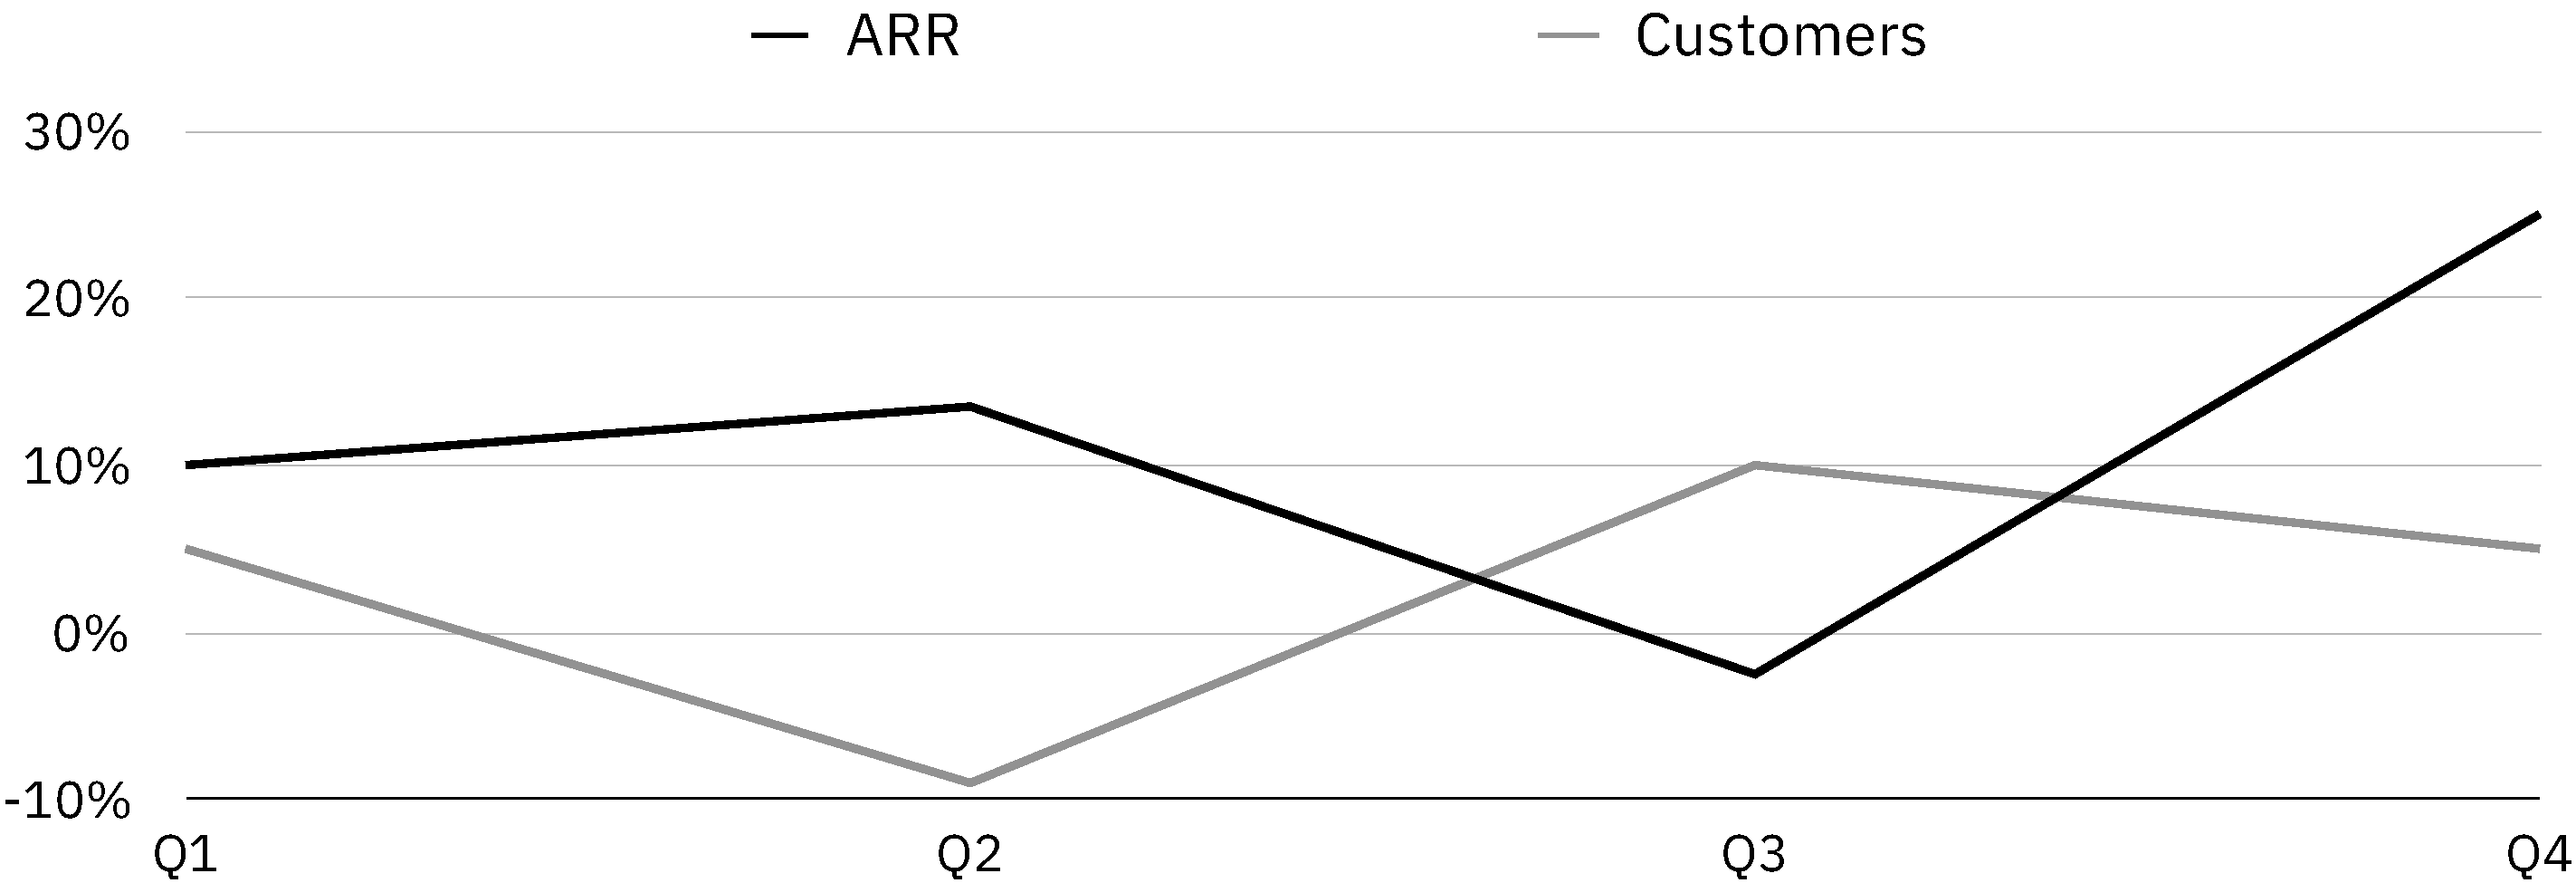
\includegraphics[width=\linewidth]{./include/ARR.pdf}
	\caption{Text block figure caption.}
	\label{fig:example} % Label for referencing this figure in the text automatically
\end{figure}

%------------------------------------------------

\begin{figure*} % Use the figure* environment for full width figures
	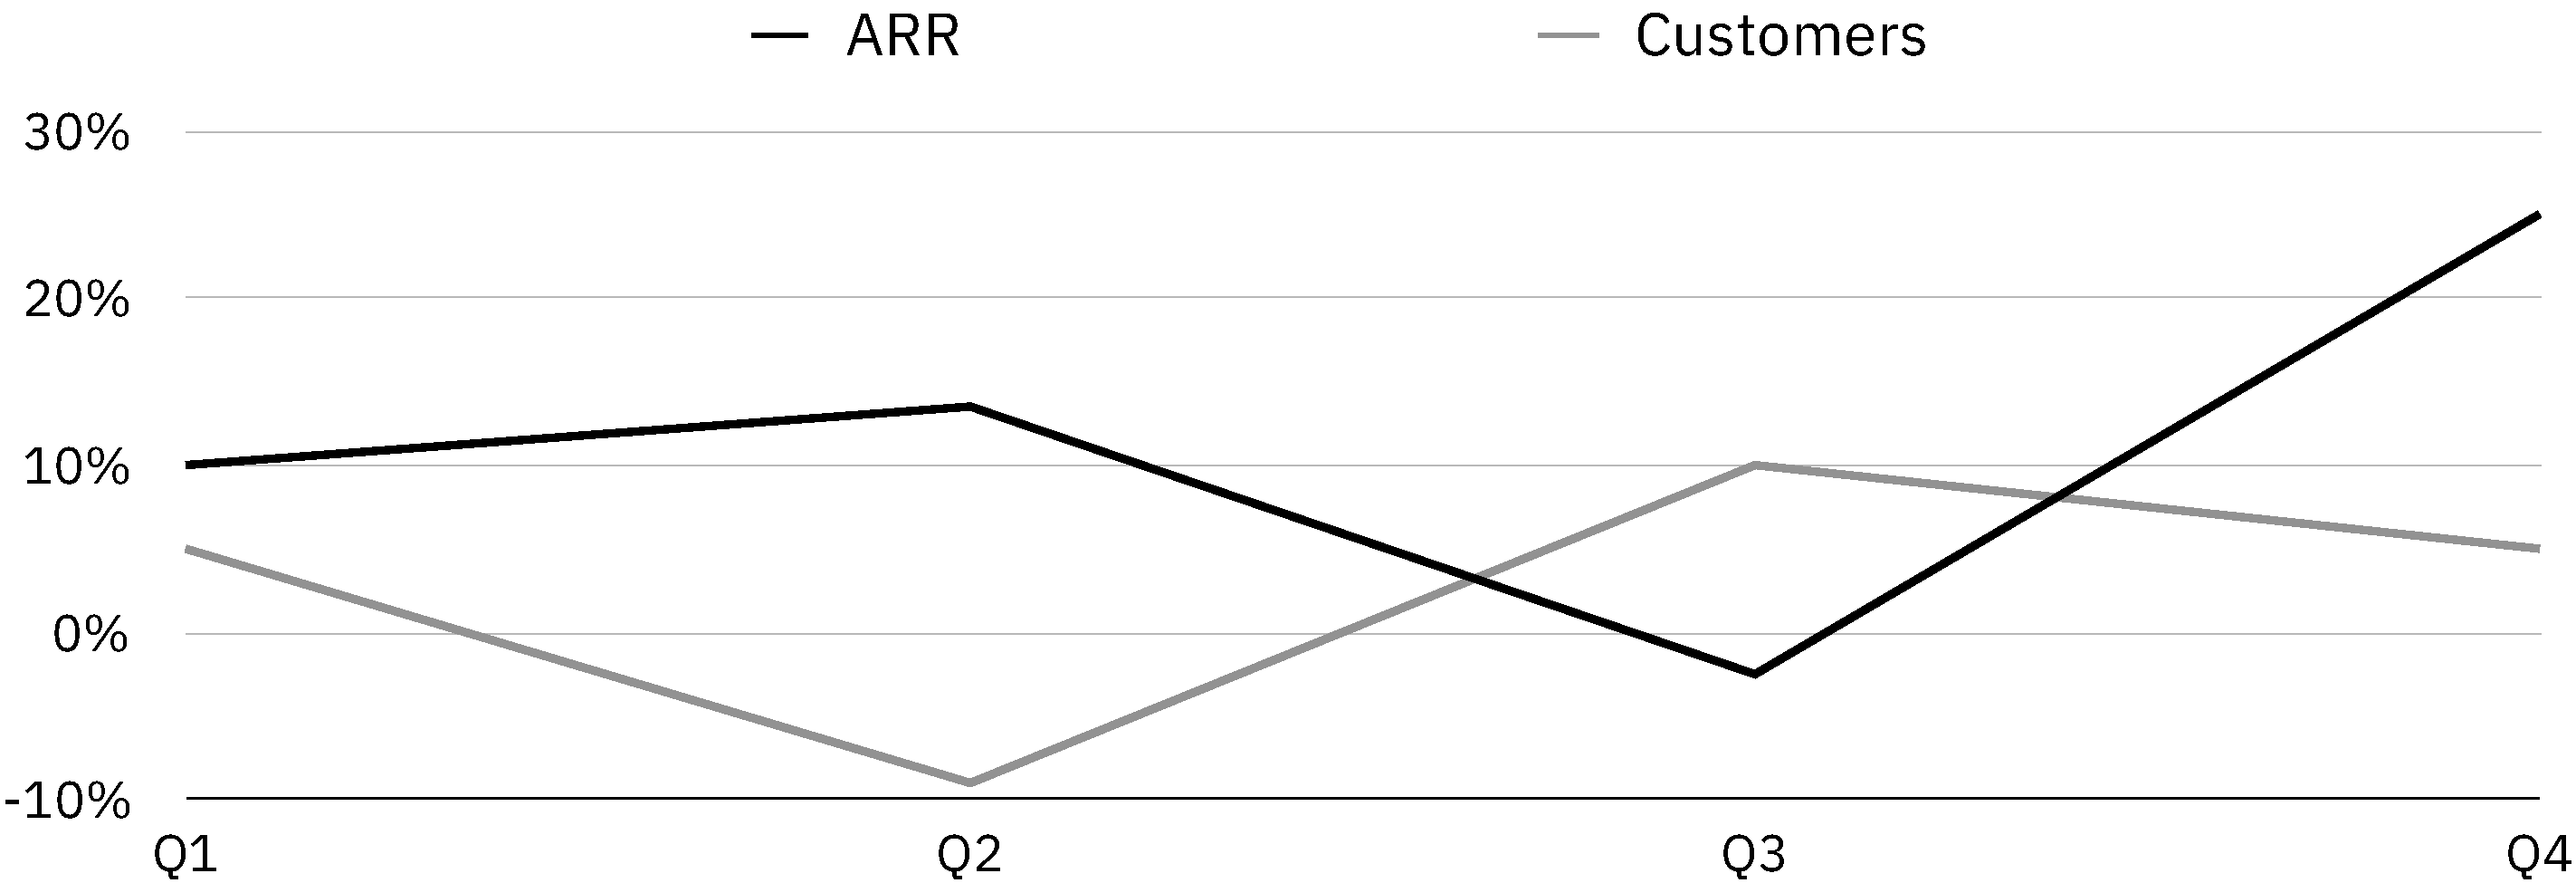
\includegraphics[width=\linewidth]{./include/ARR.pdf}
	\caption{Full width figure caption.}
\end{figure*}

%----------------------------------------------------------------------------------------
%	LISTS
%----------------------------------------------------------------------------------------

\section{List Examples}

\subsection{Bullet Point List}

\nonumsidenote{Bullet point lists can also be created in the margin. For these, we can remove the usual left margin to increase the available horizontal space:\\\medskip \begin{itemize}[leftmargin=*]\item Bullet item one. \item Bullet item two. \item Bullet item three.\end{itemize}}Lorem ipsum dolor sit amet, consectetur adipiscing elit. Praesent porttitor arcu luctus, imperdiet urna iaculis, mattis eros. Pellentesque iaculis odio vel nisl ullamcorper, nec faucibus ipsum molestie. Sed dictum nisl non aliquet porttitor.

\begin{itemize}
	\item First bullet point item
	\begin{itemize}
		\item First indented bullet point item
		\item Second indented bullet point item
		\begin{itemize}
			\item First second-level indented bullet point item
			\item Second second-level indented bullet point item
		\end{itemize}
		\item Third indented bullet point item
	\end{itemize}
	\item Second bullet point item
	\item Third bullet point item
\end{itemize}

Etiam vulputate arcu dignissim, finibus sem et, viverra nisl. Aenean luctus congue massa, ut laoreet metus ornare in. Nunc fermentum nisi imperdiet lectus tincidunt vestibulum at ac elit. Nulla mattis nisl eu malesuada suscipit.

%------------------------------------------------

\subsection{Numbered List}

\nonumsidenote[-2.5cm]{Numbered lists can also be created in the margin. For these, we can remove the usual left margin to increase the available horizontal space:\\\medskip \begin{enumerate}[leftmargin=*]\item Numbered item one. \item Numbered item two. \item Numbered item three.\end{enumerate}}Lorem ipsum dolor sit amet, consectetur adipiscing elit. Praesent porttitor arcu luctus, imperdiet urna iaculis, mattis eros. Pellentesque iaculis odio vel nisl ullamcorper, nec faucibus ipsum molestie. Sed dictum nisl non aliquet porttitor.

\begin{enumerate}
	\item First numbered item
	\begin{enumerate}
		\item First indented numbered item
		\item Second indented numbered item
		\begin{enumerate}
			\item First second-level indented numbered item
			\item Second second-level indented numbered item
		\end{enumerate}
		\item Third indented numbered item
	\end{enumerate}
	\item Second numbered item
	\item Third numbered item
\end{enumerate}

Etiam vulputate arcu dignissim, finibus sem et, viverra nisl. Aenean luctus congue massa, ut laoreet metus ornare in. Nunc fermentum nisi imperdiet lectus tincidunt vestibulum at ac elit. Nulla mattis nisl eu malesuada suscipit.

%------------------------------------------------

\subsection{Description List}

\nonumsidenote{Description lists can also be created in the margin:\\\medskip \begin{description}\item[A1] Description item one. \item[B1] Description item two. \item[C1] Description item three.\end{description}}Lorem ipsum dolor sit amet, consectetur adipiscing elit. Praesent porttitor arcu luctus, imperdiet urna iaculis, mattis eros. Pellentesque iaculis odio vel nisl ullamcorper, nec faucibus ipsum molestie. Sed dictum nisl non aliquet porttitor.

\begin{description}
	\item[Item One] Lorem ipsum dolor sit amet, consectetur adipiscing elit. Praesent porttitor arcu luctus, imperdiet urna iaculis, mattis eros. Pellentesque iaculis odio vel nisl ullamcorper, nec faucibus ipsum molestie.
	\item[Item Two] Sed dictum nisl non aliquet porttitor.
	\begin{description}
		\item[Subitem] Maecenas consectetur metus at tellus finibus condimentum. Proin arcu lectus, ultrices non tincidunt et, tincidunt ut quam. Integer luctus posuere est, non maximus ante dignissim quis.
		\begin{description}
			\item[Subsubitem] Maecenas consectetur metus at tellus finibus condimentum. Proin arcu lectus, ultrices non tincidunt et, tincidunt ut quam. Integer luctus posuere est, non maximus ante dignissim quis.
	\end{description}
	\end{description}
	\item[Item Three] Etiam vulputate arcu dignissim, finibus sem et, viverra nisl. Aenean luctus congue massa, ut laoreet metus ornare in. Nunc fermentum nisi imperdiet lectus tincidunt vestibulum at ac elit. Nulla mattis nisl eu malesuada suscipit.
\end{description}

Etiam vulputate arcu dignissim, finibus sem et, viverra nisl. Aenean luctus congue massa, ut laoreet metus ornare in.

%----------------------------------------------------------------------------------------
%	REFERENCING CITATIONS
%----------------------------------------------------------------------------------------

\section{Referencing Citations}

This statement requires citation \autocite{Smith:2024jd}.

This statement requires multiple citations \autocite{Smith:2024jd, Smith:2023qr}.

This short citation is in the margin\sidecite{Smith:2023qr}.

This long citation is in the margin\fullsidecite{Smith:2024jd}.

This statement has an in-text citation: \textcite{Smith:2024jd}.

%----------------------------------------------------------------------------------------
%	LINKS
%----------------------------------------------------------------------------------------

\section{Link Examples}

This is a URL link: \href{https://www.duckduckgo.com}{DuckDuckGo}.\nonumsidenote{Links can be clicked in the PDF to navigate to the linked website or email address.}

This is a email link: \href{mailto:example@example.com}{example@example.com}.

This is a monospaced URL link: \url{https://duckduckgo.com}.


%----------------------------------------------------------------------------------------
%	CODE
%----------------------------------------------------------------------------------------

\section{Displaying Code}

The block below is a code listing. It displays code in an easy to use way with line numbers for quick reference to specific parts of the code.

\begin{lstlisting}
{
	"city": [
		{
			"id": 1,
			"name": "Toronto",
			"country": "Canada",
			"population": 6200000
		},
		{
			"id": 2,
			"name": "New York",
			"country": "United States of America",
			"population": 8800000
		}
	]
}
\end{lstlisting}

%----------------------------------------------------------------------------------------
%	 REFERENCES/BIBLIOGRAPHY
%----------------------------------------------------------------------------------------

\newpage

\addcontentsline{toc}{section}{Reference List} % Add the bibliography to the table of contents

\begin{twothirdswidth} % Content in this environment to be at two-thirds of the whole page width
	\printbibliography[title=Reference List] % Output the bibliography with a custom section title
\end{twothirdswidth}

%----------------------------------------------------------------------------------------
%	APPENDICES
%----------------------------------------------------------------------------------------

\newpage

\section*{Appendices}

\begin{appendices}

\section{Appendix Section}

Lorem ipsum dolor sit amet, consectetur adipiscing elit. Aliquam auctor mi risus, quis tempor libero hendrerit at. Duis hendrerit placerat quam et semper. Nam ultricies metus vehicula arcu viverra, vel ullamcorper justo elementum. Pellentesque vel mi ac lectus cursus posuere et nec ex. Fusce quis mauris egestas lacus commodo venenatis. Ut at arcu lectus. Donec et urna nunc. Morbi eu nisl cursus sapien eleifend tincidunt quis quis est. Donec ut orci ex. Praesent ligula enim, ullamcorper non lorem a, ultrices volutpat dolor. Nullam at imperdiet urna. Pellentesque nec velit eget euismod pretium.

\section{Appendix Section}

Lorem ipsum dolor sit amet, consectetur adipiscing elit. Aliquam auctor mi risus, quis tempor libero hendrerit at. Duis hendrerit placerat quam et semper. Nam ultricies metus vehicula arcu viverra, vel ullamcorper justo elementum. Pellentesque vel mi ac lectus cursus posuere et nec ex. Fusce quis mauris egestas lacus commodo venenatis. Ut at arcu lectus. Donec et urna nunc. Morbi eu nisl cursus sapien eleifend tincidunt quis quis est. Donec ut orci ex. Praesent ligula enim, ullamcorper non lorem a, ultrices volutpat dolor. Nullam at imperdiet urna. Pellentesque nec velit eget euismod pretium.

\section{Appendix Section}

Lorem ipsum dolor sit amet, consectetur adipiscing elit. Aliquam auctor mi risus, quis tempor libero hendrerit at. Duis hendrerit placerat quam et semper. Nam ultricies metus vehicula arcu viverra, vel ullamcorper justo elementum. Pellentesque vel mi ac lectus cursus posuere et nec ex. Fusce quis mauris egestas lacus commodo venenatis. Ut at arcu lectus. Donec et urna nunc. Morbi eu nisl cursus sapien eleifend tincidunt quis quis est. Donec ut orci ex. Praesent ligula enim, ullamcorper non lorem a, ultrices volutpat dolor. Nullam at imperdiet urna. Pellentesque nec velit eget euismod pretium.

\end{appendices}

%----------------------------------------------------------------------------------------

\end{document}
